\documentclass[a4paper,12pt,oneside]{book}
\usepackage[utf8]{inputenc}
\usepackage{amssymb}
\usepackage{amsmath}
\usepackage{listings}
%\usepackage{color}
\usepackage{afterpage}
\usepackage{xcolor}

\usepackage{helvet}
\renewcommand{\familydefault}{\sfdefault}

\definecolor{lightblue}{rgb}{0.68, 0.85, 0.9}
\definecolor{codegreen}{rgb}{0,0.6,0}
\definecolor{codegray}{rgb}{0.5,0.5,0.5}
\definecolor{codepurple}{rgb}{0.58,0,0.82}
\definecolor{backcolour}{rgb}{0.95,0.95,0.92}
\lstdefinestyle{mystyle}{
	backgroundcolor=\color{backcolour},
	commentstyle=\color{codegreen},
	keywordstyle=\color{magenta},
	numberstyle=\tiny\color{codegray},
	stringstyle=\color{codepurple},
	basicstyle=\footnotesize,
	breakatwhitespace=false,         
	breaklines=true,                 
	captionpos=b,                    
	keepspaces=true,                 
	numbers=left,                    
	numbersep=9pt,                  
	showspaces=false,                
	showstringspaces=false,
	showtabs=false,                  
	tabsize=2
}
\lstset{style=mystyle}
\usepackage{graphicx}
\usepackage{subcaption}
\usepackage{float}
\usepackage[export]{adjustbox}
\graphicspath{ {images/} }
\usepackage{times}
\usepackage{geometry}
\usepackage{setspace}
\usepackage{tocloft}
\usepackage{booktabs}
\usepackage{fancyhdr}
\usepackage{upgreek}
\geometry{a4paper, tmargin=4cm, rmargin=2.5cm, bmargin=2.5cm, lmargin=4cm}
\usepackage{titlesec}
\usepackage[toc,page]{appendix}

%\usepackage{cite}
\usepackage{breakcites}
%\usepackage[english]{babel}
\usepackage{hyperref}
\usepackage{textgreek}

\hypersetup{
	colorlinks=true,
%	linkcolor=blue,
%	filecolor=magenta,      
%	urlcolor=cyan,
	allcolors=magenta,
	pdftitle={Thesis - Major Project},
	bookmarks=true,
%	pdfpagemode=FullScreen,
}
%\urlstyle{same}

\titleformat{\chapter}[display]{\centering\fontsize{14pt}{18pt}\selectfont\bfseries}
{\chaptertitlename\ \thechapter}{12pt}{}
\titleformat*{\section}{\fontsize{14pt}{18pt}\selectfont\bfseries}
\titleformat*{\subsection}{\normalsize\bfseries}
\titleformat*{\subsubsection}{\normalsize\bfseries}
%\titleformat*{\paragraph}{\large\bfseries}
%\titleformat*{\subparagraph}{\large\bfseries}

\renewcommand{\cftchapleader}{\cftdotfill{\cftdotsep}} % for chapters
\renewcommand\contentsname{\fontsize{14pt}{18pt}\selectfont\sffamily\centerline{TABLE OF CONTENTS}}
\renewcommand\cftloftitlefont{\fontsize{14pt}{18pt}\selectfont\sffamily\bfseries}
\renewcommand\cftlottitlefont{\fontsize{14pt}{18pt}\selectfont\sffamily\bfseries}
\pagestyle{fancy}
\cfoot{\thepage}
\rhead{}
\lhead{}
\renewcommand{\headrulewidth}{0pt}
\renewcommand{\footrulewidth}{0pt}

%\renewcommand{\baselinestretch}{1.0}
\renewcommand{\bibname}{References}
%\setstretch{1.5}

\begin{document}
	% Change the title below to your own title E.g. \title{MYPROJECTNAME}
%	\frontmatter
	\title{B.Tech Thesis Template}
	\frontmatter
	\newgeometry{a4paper, tmargin=1in, rmargin=1in, bmargin=1in, lmargin=1.5in}
	
	\fontfamily{ptm}\selectfont
	
	\addtocontents{toc}{\textbf{Title}\hfill\textbf{Page No.}\par}
	\pagecolor{lightblue}
	\begin{titlepage}
\begin{center}
\fontsize{20pt}{1cm}\selectfont \textbf{SIMULATION OF HYBRID PLASMONIC WAVEGUIDE BASED DEVICES AND ITS APPLICATIONS}

\vspace*{1.4cm}
\fontsize{16pt}{21pt}\selectfont \textbf{A Project Report}

\vspace*{.8cm}
\fontsize{16pt}{21pt}\selectfont Submitted in Partial Fulfillment of the Requirements for the\\
Award of the Degree of

\vspace*{.8cm}
\fontsize{20pt}{0.5cm}\selectfont\textbf{Bachelor of Technology}\\

\vspace*{.3cm}
\fontsize{14pt}{0.5cm}\selectfont \textit{In}

\vspace*{.3cm}
% Insert your branch in block letters where it says BRANCH NAME
\fontsize{14pt}{21pt}\textbf{Electronics and Communication Engineering}

\vspace*{.8cm}
\fontsize{12pt}{21pt}\selectfont \textit{Submitted by}\\
% Insert your name here under Name 1 and Name 2 as well as your respective Roll Numbers.
% To insert another name add this before the } --> \\NAME 3 (ROLL NUMBER)
\fontsize{14pt}{20pt}\selectfont \textbf{Saurabh Kumar}\\
\fontsize{12pt}{15pt}\selectfont Roll No.-1604055, Enrolment No.-160709\\
\fontsize{14pt}{20pt}\selectfont \textbf{Gautam Kumar Thakur}\\
\fontsize{12pt}{15pt}\selectfont Roll No.-1604070, Enrolment No.-160798\\

\vspace*{.8cm}
\fontsize{12pt}{21pt}\selectfont \textit{Under the Supervision of}\\
\fontsize{12pt}{20pt}\selectfont \textbf{Dr. Rakesh Ranjan}\\
\fontsize{10pt}{15pt}\selectfont Assistant Professor\\

\vspace*{1.0cm}
\includegraphics[width=1.25in]{NITP-Logo}

\vspace*{.3cm}
% Insert Department Name where it says DEPARTMENT NAME
\fontsize{14pt}{16pt}\selectfont \textbf{Department of Electronics \& Communication Engineering}\\
\fontsize{14pt}{16pt}\selectfont NATIONAL INSTITUTE OF TECHNOLOGY\\PATNA-800005

\vspace*{.5cm}
% You can change the month and year here
\fontsize{12pt}{20pt}\selectfont \textbf{JUNE 2020 (2019-20)}
\end{center}
\end{titlepage}
	\afterpage{\nopagecolor}
	\input{InsideCoverPage}
	\restoregeometry
	
	\fontfamily{phv} \selectfont
	
	\phantomsection \addcontentsline{toc}{chapter}{CERTIFICATE}
	\thispagestyle{plain}
\fontfamily{phv} \selectfont
\linespread{1.5}
\begin{center}
\fontsize{14}{18}\selectfont \textbf{CERTIFICATE}
\end{center}

\vspace{0.3cm}
\noindent
% Enter the title of your project in the section where it says PROJECT NAME
\normalsize This is to certify that the project titled \textbf{SIMULATION OF HYBRID PLASMONIC WAVEGUIDE BASED DEVICES AND ITS APPLICATIONS} is a bonafide record of the work done by
%Simulation of Hybrid Plasmonic Waveguide Based Devices and Its Applications
\vspace{1.0cm}

\begin{center}
% Insert your name here under Name 1 and Name 2 as well as your respective Roll Numbers.
% To insert another name add this before the } --> \\NAME 3 (ROLL NUMBER) 
\fontsize{12pt}{20pt}\selectfont \textbf{Saurabh Kumar}\\
\fontsize{10pt}{15pt}\selectfont Roll No.-1604055, Enrolment No.-160709\\
\fontsize{12pt}{20pt}\selectfont \textbf{Gautam Kumar Thakur}\\
\fontsize{10pt}{15pt}\selectfont Roll No.-1604070, Enrolment No.-160798\\
\end{center}

\vspace{1.0cm}
\noindent
% Insert the name of your branch where it says {BRANCH NAME}
\normalsize in partial fulfillment of the requirements for the award of the degree of \textbf{Bachelor of Technology} in \textbf{ELECTRONICS \& COMMUNICATION ENGINEERING} of the \textbf{NATIONAL INSTITUTE OF TECHNOLOGY, PATNA}, during the year 2019-2020.

% Electronics \& Communication Engineering
\vspace{\fill}

\begin{tabular*}{\textwidth}{@{\extracolsep{\fill}} lc}
	 & \textbf{Dr. Rakesh Ranjan} \\
	 \addlinespace[-0.8em]
	Date: $\underline{\hspace{1in}}$ & Supervisor \\
	\addlinespace[-0.8em]
	 & Assist. Professor \\
	 \addlinespace[-0.8em]
	 & ECE Dept.\\
	 \addlinespace[-0.8em]
	 & NIT Patna - 800005
\end{tabular*}

\vspace{3.0cm}

\newpage
	\phantomsection \addcontentsline{toc}{chapter}{DECLARATION AND COPYRIGHT}
	\thispagestyle{plain}
\linespread{1.5}
\begin{center}
\fontsize{14}{18}\selectfont \textbf{DECLARATION AND COPYRIGHT}
\end{center}

\vspace{0.3cm}
\noindent
\normalsize We declare that this is our own original work and that it has not been presented and will not be presented to any other University/ Institute for a similar or any other Degree award.

\vspace{3cm}

%\noindent
\begin{tabular*}{0.75\textwidth}{@{\extracolsep{\fill}} lcc}
	
	 Author's Name (Roll No.) & Signature & Date \\
	 \addlinespace[12pt]
	 Saurabh Kumar (1604055) & : $\underline{\hspace{1.5in}}$ & $\underline{\hspace{1in}}$ \\
	 \addlinespace[12pt]
	 Gautam Kumar Thakur (1604070) & : $\underline{\hspace{1.5in}}$ & $\underline{\hspace{1in}}$ \\
\end{tabular*}

\vspace{2.0cm}
\noindent
\footnotesize
\textit{This dissertation is a copy right material protected under the Berne Convention, the copy right of 1999 and other International and National enactments, in that behalf, or intellectual property. It may not be reproduced by any means, in full or in part, except for short extracts in fair dealing, for research or private study, critical scholarly review or discourser with an acknowledgment, without written permission of the Department on both the author and NIT Patna.}

\newpage
	\phantomsection \addcontentsline{toc}{chapter}{ACKNOWLEDGEMENT}
	\thispagestyle{plain}
\linespread{1.5}
\begin{center}
\fontsize{14}{18}\selectfont\textbf{ACKNOWLEDGMENT}
\end{center}

\vspace{0.3cm}
\noindent
\normalsize We wish to express our deep sense of gratitude and indebtedness to our supervisor \textbf{Dr. Rakesh Ranjan}, Department of Electronics \& Communication Engineering, NIT Patna, for introducing the present topic and for his inspiring guidance, constructive criticism and invaluable suggestions throughout this project work.

\vspace{1.0cm}
\noindent
We also extend our sincere thanks to all our friends who have patiently helped us in accomplishing this undertaking. We also thank \textbf{Mr. Pintu Kumar} for his constant support throughout the project work.

\vspace{1.0cm}
\noindent
At last we must express our sincere heartfelt gratitude to all the staff members
of Electronics \& Communication Engineering Department who helped us directly or
indirectly during this course of work.

\vspace{\fill}
\begin{tabular*}{\textwidth}{@{\extracolsep{\fill}} cc}
	Date: \hspace{1pt} $\underline{\hspace{1in}}$
	& \textbf{Saurabh Kumar} \\
	\addlinespace[-0.8em]
	& (1604055) \\
	\addlinespace[-0.8em]
	Place: $\underline{\hspace{1in}}$ & \\
	\addlinespace[0.8em]
	& \textbf{Gautam Kumar Thakur} \\
	\addlinespace[-0.8em]
	& (1604070) \\
	& ECE Department \\
	\addlinespace[-0.8em]
	& National Institute of Technology \\
	\addlinespace[-0.8em]
	& Patna - 800005
\end{tabular*}

\vspace{2cm}
\newpage
	\phantomsection \addcontentsline{toc}{chapter}{DEDICATION}
	\thispagestyle{plain}
%\begin{center}
%\textbf{DEDICATION}
%\end{center}


\clearpage
\normalsize
\begin{center}
	\thispagestyle{empty}
	\vspace*{\fill}
	Dedicated to all those people who supported us throughout this project.
	\vspace*{\fill}
\end{center}
\clearpage

\newpage
	
	
	\phantomsection \addcontentsline{toc}{chapter}{ABSTRACT}
	\thispagestyle{plain}
\linespread{1.5}
\begin{center}
	\fontsize{14}{18}\selectfont \textbf{ABSTRACT}
%	\textbf{\textbf{\fontsize{14pt}{24pt}\selectfont ABSTRACT}}
\end{center}

\vspace{0.3cm}

% Start typing out your abstract after the \selectfont tag. And after your last line add a \\ if you require more spacing

%\fontsize{12pt}{18pt}\selectfont 
\normalsize
\noindent
This project aims to the study of hybrid plasmonic waveguides (HPWs) and their potential applications in the field of photonics. Here, we have presented our effort toward recent advancement in the photonic integrated circuits and related studies. We have simulated various types of HPW structures, proposed over past few years and studied their characteristics such as effective mode index, mode effective area, and propagation length. It is observed that there is a trade-off between mode confinement and propagation loss in case of most of the HP-waveguides. Structures with smaller mode effective area tend to have larger propagation loss and vice-versa.

Further, we have investigated a few potential applications of HP-waveguides such as optical ring resonators (ORR) and optical nanoantenna. We have simulated a hybrid dielectric-loaded plasmonic waveguide (HDLW) based ring resonator and studied its transmission characteristics at both constructive and destructive interference wavelengths. A high extinction ratio of 22.5 dB and 24.9 dB is obtained at r = 2 $\upmu \text{m}$ and 5 $\upmu \text{m}$ respectively. While low transmission loss of 0.8 dB and 0.5 dB is obtained at radii 2 $\upmu \text{m}$ \& 5 $\upmu \text{m}$ respectively. For nanoantenna, we have studied the characteristics of a HP-waveguide horn-nanoantenna and simulated its input HP-waveguide which is based on silicon-on-insulator (SOI) configuration. All simulations have been carried out using finite element method (FEM) in the COMSOL Multiphysics simulation software and graphs are plotted with the help of MATLAB.


\newpage

	
	\setstretch{1.5}
	
	
	\phantomsection \addcontentsline{toc}{chapter}{TABLE OF CONTENTS}
	\tableofcontents
	\newpage
	\phantomsection \addcontentsline{toc}{chapter}{LIST OF FIGURES}
	\listoffigures
	\newpage
	\phantomsection \addcontentsline{toc}{chapter}{LIST OF TABLES}
	\listoftables
	 
	\mainmatter
	
	
	\chapter{Introduction}
	%---------------------------CHAPTER - 01----------------------------
%\linespread{1.5} 
\normalsize
In recent years, increasing demand of high data-rate devices and ultra-compact integrated circuits have pulled researcher's interest towards optical fiber communication. It is observed that state of the art optical devices tends to have bandwidth in terahertz region and can operate at very high frequencies. As the demand of high data-rate devices is increasing significantly in day-to-day life, world is becoming more reliant on optical communication than the electronics communication system. Many signal processing devices are being replaced by optical devices. Usually optical devices tend to have bandwidth in terahertz range.

Plasmonic waveguides and waveguide-based components are considered as the ideal candidates for highly integrated nanoscale photonic electronic circuit applications~\cite{Barnes2003,Ozbay2006}. Different kinds of plasmonic waveguiding structures have been proposed and developed in recent years, including metallic strips and nanowires, coupled nanowires, metallic grooves, metal-insulator-metal (MIM) waveguides ~\cite{Feng2007}, dielectric-loaded plasmonic waveguides ~\cite{Reinhardt2009,Hong2009}, as well as hybrid plasmonic waveguides ~\cite{Wang2019,Nikoufard2017,Hong2010,Oulton2008}.

\section{Plasmonic Waveguides}
The conventional dielectric waveguides which works on the principle of total internal reflection at the core/cladding interface, tend to suffer from diffraction limit. As a consequence, the minimum core size of conventional dielectric waveguides is of the order of the wavelength of light, posing a fundamental limit to the size scaling of integrated optical chips~\cite{Feng2007}. However, several schemes have been already proposed in order to transport optical information over long distances by means of deep subwavelength modes~\cite{Ohtsu2002,Takahara2004}.

Recently, dielectric slot-waveguide structures have been proposed, able to confine light fields over nanoscale low-refractive-index dielectric regions~\cite{Almeida2004,Feng2006,Xu2004}. These structures are based on nanoscale regions sandwiched by high-refractive-index dielectrics. It has been shown that, depending on the actual design characteristics, deep subwavelength localization and sizeable field-enhancement effects can be achieved due to the large-refractive-index discontinuity at the dielectric boundary regions. An alternative approach to achieve high field confinement is based on the excitation of surface plasmon polaritons (SPPs) in metal/dielectric waveguide structures. SPPs are surface localized light waves at dielectric–metal interfaces which are coupled to free electron oscillations in the metal.

\section{Hybrid Plasmonic Waveguides}
The hybrid plasmonic waveguides have drawn substantial research interest because of the exciting potential for integrating metallic and semiconductor nanostructures to fully exploit the advantages of both metals (light concentration and high electrical conductivity) and semiconductors (light emission and photocurrent generation). Moreover, the presence of a high refractive index semiconductor, separated from the metal film by a low refractive index layer, yields the best trade-off between the propagation loss and the power confinement ~\cite{Oulton2008}. Several hybrid plasmonic waveguide structures have been proposed and discussed both in theory and experiment; they include hybrid dielectric-loaded and doubled-hybrid plasmonic waveguide~\cite{Oulton2008,Hong2010}. Among these kinds of waveguide, the hybrid dielectric-loaded plasmonic waveguide (HDPW) has received particular attention as a transmission medium for various plasmonic components of high optical performance, such as waveguide-bends and couplers, as well as lasers at a deep sub-wavelength scale. Moreover, the HDPW structures have no minimum thickness limitation of the low refractive index layer, and thus achieve higher confinement while minimizing the scattering losses by virtue of their smoother layer interfaces.

Over past few years, HPW has been used for variety of applications. Our study here is restricted only to optical ring resonators (ORR) and optical nanoantennas.

\subsection{Optical Ring Resonator}
Ring resonators play an important role in the success of silicon photonics, because silicon enables ring resonators of an unprecedented small size. A generic ring resonator consists of an optical waveguide which is looped back on itself, such that a resonance occurs when the optical path length of the resonator is exactly a whole number of wavelengths. Ring resonators therefore support multiple resonances, and the spacing between these resonances, the free spectral range (FSR), depends on the resonator length. As discussed in~\cite{Bogaerts2011}, for many applications it is preferred to have a relatively large FSR (several nm), and this implies the use of small rings. This translates into a very hard requirement for the optical waveguide: to make a compact ring, a small bend radius is required, and this in turn is only possible with high-contrast waveguides with strong confinement.

A ring resonator as a stand-alone device only becomes useful when there is a coupling to the outside world. The most common coupling mechanism is using codirectional evanescent coupling between the ring and an adjacent bus waveguide. As will be discussed in more detail in the next section, the transmission spectrum of the bus waveguide with a single ring resonator will show dips around the ring resonances. This way, the ring resonator behaves as a spectral filter, which can be used for applications in optical communication, especially wavelength division multiplexing (WDM).

In this project, we have studied the characteristics of optical ring resonator (ORR) based on two different types of HPW structures; hybrid dielectric-loaded plasmonic waveguides (HDLW)~\cite{Hong2011} and hybrid metal-insulator-metal (HMIM) plasmonic waveguide~\cite{PSharma2016}. The HDLW based resonator structure consists of SOI-configuration with silica (SiO$_2$) as low refractive index layer and silver (Ag) as metal layer. While HMIM waveguide-based resonator consists of Aluminum Gallium Arsenide (AlGaAs) and poly tetra fluoro ethylene (PTFE) as high and low dielectric layer respectively.

\subsection{Optical Nanoantenna}
Optical nanoantenna efficiently convert free-propagating optical radiation into localized energy and vice versa. Therefore, the potential applications of optical antenna are closely related to their ability to strongly localized optical fields likewise; scattering, sensing inter- and/or intra- chip communications. Moreover, optical nanoantenna can play a vital role in reducing power consumption and allow higher speed for on-chip optical interconnects. As a result, it is considered as a prominent alternative to optical waveguide-based interconnects for on-chip wireless communication with high spectral efficiency.

Designing of a nanoantenna for wireless optical communication involves the basic principle: optimization of shape in order to match the impedance. It also takes into account for the parameters of antenna likewise; gain, directivity and reflection-coefficient.

In this context, we have studied the characteristics of horn-nanoantenna with silicon-on-insulator (SOI) configuration ~\cite{Nourmohammadi2019,Nikoufard2018}. It is able to operate in a range of optical frequencies by using a SOI-based horn-shaped nanoantenna. This nanoantenna is broadband at a wider range of frequencies (160–400 THz) in comparison with the previous antennas. This nanoantenna is capable of radiating all three optical communication wavelengths of 1550 nm (193.5 THz), 1310 nm (229 THz) and 850 nm (352.9 THz) with slightly higher gains at all wavelengths and smaller dimensions. All these features make this nanoantenna a good candidate for energy-harvesting applications or integration with devices such as dual laser combiner modules in communication systems. The horn nanoantenna has also been explored for several applications in near-infrared, far-infrared and visible region.
	\chapter{Literature Review}
	%\linespread{1.5} 
\normalsize
\section{Literature Review on HPW}
In recent years, hybrid plasmonic waveguides have been a demanding area of research in photonics. One of the main reasons for the increasing demand of the hybrid plasmonic waveguide is that its ability to confine light at nanoscale with long range propagation. In past decade, researchers have studied HPW for number of applications. Some of them are documented in the literature~\cite{Oulton2008,Hong2011,Alam2015,Tsilipakos2016,PSharma2016,Nikoufard2017,Nikoufard2018,Nourmohammadi2019,Wang2019,PKumar2020}. These authors have utilized different properties of hybrid plasmonic waveguides for various applications.

\cite{Oulton2008} proposed a dielectric nanowire-based structure to achieve long range propagation with subwavelength confinement. In this structure, a dielectric nanowire is separated from a metal surface by a nanoscale dielectric gap such that the 'capacitor-like' energy storage is enabled by the coupling between the plasmonic and waveguide modes across the gap.

\cite{Hong2011} analyzed a hybrid dielectric-loaded plasmonic waveguide for long range propagation and strong field confinement. They explored this structure to study the characteristics of various wavelength selective components for high optical performance.

\cite{Alam2015} utilized the properties of the mode supported by hybrid plasmonic waveguides. Considering silicon compatibility of the HPW, a number of hybrid waveguide devices were presented for silicon on insulator (SOI) platform.

\cite{Tsilipakos2016} proposed a disk resonator based on hybrid plasmonic waveguide for Kerr bistability and self-pulsation, operating with mW input powers. They attempted to reduce the input power requirement for various devices in silicon photonics.

\cite{PSharma2016} analyzed the mode properties of a two layered HP-waveguide based on metal-insulator-metal (MIM) configuration and compared the results with that of single layered HP-waveguide. To understand the mode confinement of both waveguides, mode effective areas of both structures were compared. Further, a ring resonator based on hybrid metal-insulator-metal (HMIM) waveguide was simulated and its transmission characteristics were studied.

\cite{Nikoufard2017} studied the mode properties of InP-based deeply etched HP-waveguide and compared the results with that of InP-based conventional waveguide. Utilizing various properties of InP-based deeply etched HP-waveguide, a nanoscale multimode interference (MMI) power splitter was proposed. The effect of various MMI parameters such as length, width, and wavelength on optical power transmission was investigated. Further, ~\cite{Nikoufard2018} utilized InP-based HP-waveguide to propose a bowtie nanoantenna with the capability of monolithic integration with laser and photodetector.

\cite{Nourmohammadi2019} proposed a horn-shaped nanoantenna for broadband nanophotonic applications. This structure utilized a HP-waveguide with SOI-configuration. It was observed that proposed structure is able to operate in a wide optical frequency range of 160--400 THz and includes optical communication wavelengths of 850, 1310 and 1550 nm.

\cite{Wang2019} proposed a silicon-based HP-waveguide with the goal of obtaining long range propagation at optical communication wavelength of $\lambda$ = 1550 nm. This structure is designed with SOI-rib and a metal cap at the top. Some potential applications for the proposed structure were investigated.

\cite{PKumar2020} investigated a multi-layered hybrid metal-insulator-metal plasmonic waveguide which was observed to have a relatively smaller mode effective area in the low-dielectric region at optical communication wavelength of 1550 nm. Adding further to that, proposed structure was explored for crosstalk estimation.

Although most of the authors in their recent work shown that hybrid plasmonic waveguide poses tremendous qualities in terms of subwavelength confinement, few authors have pointed out that it tends to suffer from large loss. So, there is a trade-off between confinement and loss which limits the capability of hybrid plasmonic waveguides at some extent.
	\chapter{Theoretical Discussion of HPW and Nano-Antenna}
	%\linespread{1.5} 
\normalsize
In this chapter, we discuss the physics and working principle of surface plasmon polaritons (SPPs), plasmonic waveguides and applications of hybrid plasmonic waveguides (HPWs). We also discuss some HPW based devices such as, optical ring resonators and optical nanoantennas.

\section{Surface Plasmon Polaritons}
With the rapid development of optical techniques, data transmission systems require highly increasing integration of photonic devices. It is estimated that the data transmission rates will reach 10 Tbit $\text{s}^{-1}$ by decreasing the element size of the photonic devices to the nanometer scale; in this case, the data storage density will be as high as 1 Tbit $\text{inch}^{-1}$. However, it is very difficult for conventional photonic devices to reduce the element sizes to the nanometer scale because of Abbe’s diffraction limit to about one-half of the optical wavelength. Excitation of surface plasmon polaritons (SPPs) can overcome the diffraction limit and offer a promising approach to control and manipulation propagation and dispersion of light on the nanometer scale. SPP is an electromagnetic excitation existing at the interface between a metal and a dielectric material; furthermore, the resonant interaction between the SPP and the electromagnetic radiation at metallic interfaces results in a remarkably enhanced optical near-field~\cite{Zhang2012,Atwater2007}.

\subsection{Physics of Surface Plasmon Polaritons}
\subsubsection{Excitation}
SPPs are surface electromagnetic waves that propagate along the interface between a metal and a dielectric material, and the surface electromagnetic waves consist of surface charges. First of all, how to excite the surface charges? We consider a p-polarized wave (TM mode, the electric field vector parallel to the incident plane) that reaches a smooth planar interface at an incident angle $\theta_1$. The incident wave has a photon momentum $hk_d$ (where $k_d = 2\pi n_d/\lambda$) in the dielectric with a refractive index $n_d$. When the wave arrives at the interface, the reflective wave will propagate along the direction with an angle equal to the incident angle, and the photon momentum is conserved.

\subsubsection{Coupling}
The interaction between the electromagnetic field and the surface charges results in an increase in the SPP momentum compared with that of the free space according to the SPP dispersion relation given in~\cite{Zhang2012}, which gives rise to the momentum mismatch between light and SPP. The momentum of light and SPP can be matched using different coupler configurations such as prism couplers ~\cite{Zayats2005,Zayats2003}, grating couplers~\cite{Zayats2005,Zayats2003}, fiber and waveguide couplers ~\cite{Homola1999,Riziotis2009,Abdulhalim2008,Sharma2007}.

The metal film is illuminated through the dielectric prism at an angle of incidence greater than the critical angle or the total internal reflection angle in the Kretschmann configuration~\cite{Kretschmann1968}. The light wavevector increases in the optically dense medium at a certain incident angle larger than the critical angle. The in-plane component of the light wavevector in the prism coincides with the SPP wavevector on an air–metal surface, which gives rise to the light tunneling through the metal film, and as a result, the light is coupled to the SPP. Furthermore, the efficiency of SPP excitation decreases with increasing film thickness due to the increase in the tunneling distance.

\subsubsection{Propagation}
Once light has been converted into an SPP mode on a flat metal surface it will propagate, but will gradually attenuate owing to losses arising from absorption in the metal. The propagation length of the SPP is thereby limited by the imaginary part of the complex SPP wavevector $k_{\text{spp}}$ due to the internal damping (ohmic losses), where $k_{\text{spp}} = k_{\text{sppr}} + \text{i}k_{\text{sppi}}$. Based on the SPP dispersion relation given in~\cite{Zhang2012}, the propagation length of SPP $\delta_{\text{spp}}$ is given by~\cite{Barnes2003,Bozhevolnyi2001} \newline \[\delta_{\text{spp}} = \dfrac{1}{2k_{\text{sppi}}} = \dfrac{\lambda}{2\pi} \bigg(\dfrac{\varepsilon_{\text{mr}} + \varepsilon_{\text{d}}}{\varepsilon_{\text{mr}}\varepsilon_{\text{d}}}\bigg)^{3/2}\dfrac{\varepsilon_{\text{mr}}^2}{\varepsilon_{\text{mi}}}\] \newline
where $\varepsilon_{\text{mr}}$ and $\varepsilon_{\text{mi}}$ are the real and imaginary parts of the dielectric function of metal, respectively, that is, $\varepsilon_{\text{m}} = \varepsilon_{\text{mr}} + \text{i} \varepsilon_{\text{mi}}$, and $\delta_{\text{spp}}$ is the distance after which the SPP intensity decreases to $1/e$ of its starting value.

\subsection{Applications of SPPs}
Controlling light on scales much smaller than the light wavelength can be achieved by excitation of SPPs, owing to their unique optical properties described above. SPPs exhibit potential applications in subwavelength optics.

\section{Plasmonic Waveguides}
In this section, we consider plasmonic waveguides from the point of view of
the longitudinal-transverse waveguide decomposition. Unlike the asymmetric dielectric waveguide, a very significant difference being that in the plasmonic case at least one of the layers is metallic with a dielectric constant having negative real-part in the operating frequency range (typically, infrared to optical)~\cite{Orfanidis2002}. A typical plasmonic waveguide consisting of a thin film $\varepsilon_f$, sandwiched between a cladding cover $\varepsilon_c$ and a substrate $\varepsilon_s$ is shown in Fig.~\ref{fig:pwg_struc}. In general, plasmonic waveguides are classified into three categories: (a)single interface between a dielectric $\varepsilon_c$ and a metal $\varepsilon_f$ , (b) metal-dielectric-metal (MDM) configuration in which $\varepsilon_f$ is a lossless dielectric and $\varepsilon_c$, $\varepsilon_s$ are metals, (c) dielectric-metal-dielectric (DMD) configuration in which $\varepsilon_f$ is a metal and $\varepsilon_c$, $\varepsilon_s$ are lossless dielectrics.

\begin{figure}
	\centering
	\includegraphics[width=.8\textwidth]{plasmonic_wg}
	\caption{Plasmonic waveguide depicting TM modes in either a DMD or MDM configuration~\cite{Orfanidis2002}.}
	\label{fig:pwg_struc}
\end{figure}

Here, the quantities $\varepsilon_c$, $\varepsilon_f$, $\varepsilon_s$ denote the relative permittivities of the media, that is, $\varepsilon_i$ = $\epsilon_i / \epsilon_0$, $i = c, f, s$, where $\epsilon_i$ is the permittivities of the $i^{th}$ medium and $\epsilon_0$, the permittivity of vacuum.

\subsection{Single Metal-Dielectric Interface}
The case of a single metal-dielectric interface can be thought of as the limit of a DMD configuration when the film thickness tends to infinity, $a \to \infty$. It is depicted in Fig.~\ref{fig:smd_struc}

\begin{figure}
	\centering
	\includegraphics[width=.8\textwidth]{smd_pwg}
	\caption{Surface plasmon wave propagating along metal-dielectric interface.~\cite{Orfanidis2002}.}
	\label{fig:smd_struc}
\end{figure}

\subsection{Metal-Dielectric-Metal Configuration}
An MDM waveguide consists of a single dielectric layer sandwiched between two metal layers~\cite{Maier2007}. Because of the predicted attractive properties of MDM waveguides, their modal structure has been studied in great details~\cite{Kocaba2009}, and people have also used MDM for many applications~\cite{Veronis2009}.

\subsection{Dielectric-Metal-Dielectric Configuration}
Another possible structure of an SPP waveguide would consist of a thin metal film surrounded by two dielectric claddings or a thin metal film completely embedded in one dielectric material. Such a structure supports both short-range surface plasmon-polaritons (SRSPPs) and long-range surface plasmon-polaritons (LRSPPs). The latter are preferred for waveguiding purposes. With respect to this dielectric–metal–dielectric structure, two figures of merit, namely the propagation length and confinement, have been the focus of recent publications~\cite{Sellai2008}.

\section{Hybrid Plasmonic Waveguides}
In general, the hybrid plasmonic waveguide (HPW)~\cite{Alam2013,Hong2010,Oulton2008,Noghani2013,Bhaumik2016,Zeng2011} consists of a metal surface separated from a high-index slab by a low-index spacer. In this structure, the power is highly concentrated in the low-index spacer layer. In recent years, various structures of HPW have been proposed. Also, these structures are used for number of applications. Some of the applications of HPW are already mentioned in the previous chapter.

\subsection{Modes Supported by HPW}
In case of coupling between two identical waveguides, one of the coupled modes exhibits even symmetry and the other one exhibits odd symmetry with respect to the midpoint of the gap region (spacer) separating the two guides. In case of coupling between two dissimilar waveguides (the case discussed in this study), the coupled modes lack complete symmetry but as shown later in this section, one of the modes is still “quasieven” (does not become zero anywhere in the spacer region) and the other mode is “quasi-odd” (becomes zero somewhere in the spacer region)~\cite{Alam2013}.

\subsection{Hybrid Plasmonic Waveguide Structures}
In order to understand the properties and working of HP-waveguides, we have studied and simulated various structures proposed in recent literature. Some of those structures are briefly discussed in this section.

\subsubsection{Silicon-based HPW with Metal Cap}
\label{subsubsec:nslc_shpw}
Fig.~\ref{fig:shpw_mc_struc} shows the cross section of the Si-based HP-waveguide structure, which consists of a SOI rib with a metal cap. For such a structure, the fabrication is simple and CMOS compatible. One could use a standard SOI wafer. An alternative way is using the method of depositing SiO$_2$ and alpha-Si thin films on a Si substrate with the PECVD (plasma enhanced chemical vapor deposition) technology~\cite{Dai2006}.

When the thickness of the SiO$_2$ layer between Si and metal is large (e.g., 0.5 $\upmu$m), the fundamental mode field is confined well in the Si region and the metal layer almost does not influence the mode field distribution. In this case, the present structure is like a regular SOI nanowire. However, when the SiO$_2$ thickness becomes smaller (e.g., <50 nm), the metal layer will introduce a significant influence on the field distribution of the guided mode.

\begin{figure}
	\centering
	\includegraphics[width=1\textwidth,height=0.3\textheight]{shpw_mc_struc.jpg}
	\caption{Cross-section of Si-based HP-waveguide with metal cap.}
	\label{fig:shpw_mc_struc}
\end{figure}

\subsubsection{HMIM Plasmonic Waveguide}
\label{subsubsec:hmim_pw}
HMIM (hybrid metal-insulator-metal) contains a set of insulators sandwiched between two metal layers, where set of insulators contains three dielectric layers; high dielectric in between two low dielectric layers. Energy will be guided through two layers of low dielectrics, due to the coupling behavior of plasmonic and hybrid modes. Fig.~\ref{fig:hmim_struc} shows the cross-section of HMIM waveguide.

\begin{figure}[!t]
	\centering
	\includegraphics[width=0.5\textwidth,height=0.3\textheight]{hmim_struc.jpg}
	\caption{Cross-section of HMIM waveguide.}
	\label{fig:hmim_struc}
\end{figure}

\subsubsection{InP-based Hybrid Plasmonic Waveguide}
\label{subsubsec:InP_hpw}
The lateral cross-section of deeply-etched conventional and hybrid plasmonic waveguides on an InP substrate are shown in Fig.~\ref{fig:InP_hpw_struc}.

\begin{figure}
	\centering
	\includegraphics[width=0.5\textwidth,height=0.3\textheight]{InP_hpw_struc.jpg}
	\caption{Cross-section of InP-based HP-waveguide.}
	\label{fig:InP_hpw_struc}
\end{figure}

\section{Hybrid Plasmonic Waveguide Devices}
As already mentioned in the previous chapter, hybrid plasmonic waveguides are used to fabricate number of devices used in photonic integrated circuits~\cite{Alam2015}. Here, we have presented our effort toward the study of hybrid plasmonic waveguide based optical ring resonators and optical nanoantenna.

\subsection{Ring Resonators}
In general, a ring resonator consists of a looped optical waveguide and a coupling mechanism to access the loop. When the waves in the loop build up a round trip phase shift that equals an integer times 2$\pi$, the waves interfere constructively and the cavity is in resonance~\cite{Bogaerts2011,Bogaerts2006,Heebner2008}.

In its simplest form a ring resonator can be constructed by feeding one output of a directional coupler back into its input, the so-called all-pass filter (APF) or notch filter configuration. The term ring resonator is typically used to indicate any looped resonator, but in the narrow sense it is a circular ring. When the shape is elongated with a straight section along one direction (typically along the coupling section) the term racetrack resonator is also used. We will use ring resonator throughout this paper, but most derivations and results apply to racetracks and loops of other shapes.

\subsubsection{HDLW based Ring Resonator}
Given the advantages of the hybrid dielectric-loaded plasmonic waveguide, we have used it to build a ring resonator. It is formed by a ring waveguide placed in the proximity of a straight bus waveguide Fig.~\ref{fig:hdlw_geom} to allow optical coupling between them. A portion of the optical power propagating in the straight waveguide (propagating mode) is coupled to the ring and excites a circulating mode of the RR. The efficiency of this coupling depends on the gap between the ring and the straight waveguide and on the radius of the RR. The interference between the circulating mode and the propagating mode in the straight waveguide results in the filter properties of the RR, which are characterized by the extinction ratio and the FSR. The extinction ratio of the RR (defined as the ratio between the minimum and maximum transmission outputs) is determined by the strength of the coupling between the ring and the straight waveguide sections and by the attenuation of the plasmonic wave propagation, as well as the bend loss around
the ring~\cite{Hong2011}.

\begin{figure}
	\centering
	\includegraphics[width=.8\textwidth]{hdlw_geom}
	\caption{3D view of HDLW based ring resonator}
	\label{fig:hdlw_geom}
\end{figure}

\subsection{Optical Nanoantennas}
Nanoantennas are the counterpart of antennas at microwave and radio frequencies (RF), which are designed to convert free-propagating electromagnetic radiation into localized electric currents, and vice versa. It has become an emerging field in the recent decade with the rapid growth of nano-fabrication technologies, which provide the feasibility of squeezing the fabrication resolution down to the nanometer range with top-down approaches, enabling fascinating nano-optoelectronic devices at visible frequencies. Aside from their transmitting and receiving functionality, the operation of nanoantennas differs dramatically from their RF counterparts, and their analysis and design rules should accordingly be modified.

\subsubsection{SOI-based HP-waveguide Horn Nanoantenna}
The structure of nanoantenna consists of a SOI-based hybrid plasmonic waveguide that is connected to a horn-like configuration. A schematic of the horn nanoantenna is shown in Fig.~\ref{fig:hnano_geom}. As seen, the layer structure of the waveguide and horn-nanoantenna are the same, so this configuration is suitable for monolithic integration with the SOI-based passive photonic integrated circuits. In addition, the layer stack used in the proposed nanoantenna is compatible with the complementary metal-oxide-semiconductor (CMOS) technology which makes the fabrication of the proposed device feasible. The horn-nanoantenna is an ellipsoidal configuration which is connected to the hybrid plasmonic (HP) waveguide.

% The [H] after {figure} fixes the positioning of images.
\begin{figure}[H]
	\centering
	\includegraphics[width=.8\textwidth]{hnano_geom}
	\caption{3D view of horn nanoantenna}
	\label{fig:hnano_geom}
\end{figure}

	\chapter{Simulation Result and Comparisons}
	%\linespread{1.5} 
%\normalsize
This chapter contains all the simulation results and graph plots for different parameters and adequate discussion on the obtained results. All structures are simulated in wave optics module of COMSOL Multiphysics software and graphs are plotted with the help of MATLAB.

\section{HPW Structures}
We have simulated three different structures of hybrid plasmonic waveguides: InP-based deeply etched HPW, hybrid metal-insulator-metal (HMIM) plasmonic waveguide and hybrid dielectric-loaded plasmonic waveguide (HDLW). We have also studied some characteristics and properties of these structures such as propagation length and effective mode index at different widths and thicknesses of the waveguides.

\subsection{Silicon-based HPW with Metal Cap}
The simulation results of HPW structure discussed in Section~\ref{subsubsec:nslc_shpw} are shown in this section. Fig.~\ref{fig:nslc_mode_profile} shows the field distribution of the major-component $E_\text{y}$ of the electrical fields. From these figures, one sees that there is more optical confinement in the Si layer when the core width increases. This is why the effective index real($n_\text{eff}$) and the propagation distance $L_\text{prop}$ increases as the core width increases, as shown in Fig.~\ref{fig:nslc_neffr} and ~\ref{fig:nslc_proplen}, respectively. We also see that the thickness $h_\text{SiO2}$ of the $\text{SiO}_2$ nano-layer plays an important role for the propagation distance. When choosing a thinner $\text{SiO}_2$ layer, the propagation distance becomes smaller. For the case with a relatively large thickness $h_\text{SiO2}$ (e.g., 50 nm), more power confined in silicon region. Therefore, when the core width decreases, the power confined in the silicon region will change greatly. This is why the influence of the core width on the propagation distances is significant when the thickness $h_\text{SiO2}$ is relatively large.

\begin{figure}[!t]
	\centering
	\includegraphics[width=1\textwidth]{shpw_mc_mode.jpg}
	\caption{Field distribution of the major component $E_\text{y}$ of the quasi-TM fundamental mode for the cases of $w_\text{co}$ = 100nm, 300nm, and 500nm.}
	\label{fig:nslc_mode_profile}
\end{figure}

\begin{figure}[!t]
	\centering
	\includegraphics[width=1\textwidth]{nslc_neffr_eps}
	\caption{The real part of the effective refractive index $n_\text{eff}$ for $h_\text{SiO2}$ = 5nm, 20nm, and 50nm.}
	\label{fig:nslc_neffr}
\end{figure}

\begin{figure}[!t]
	\centering
	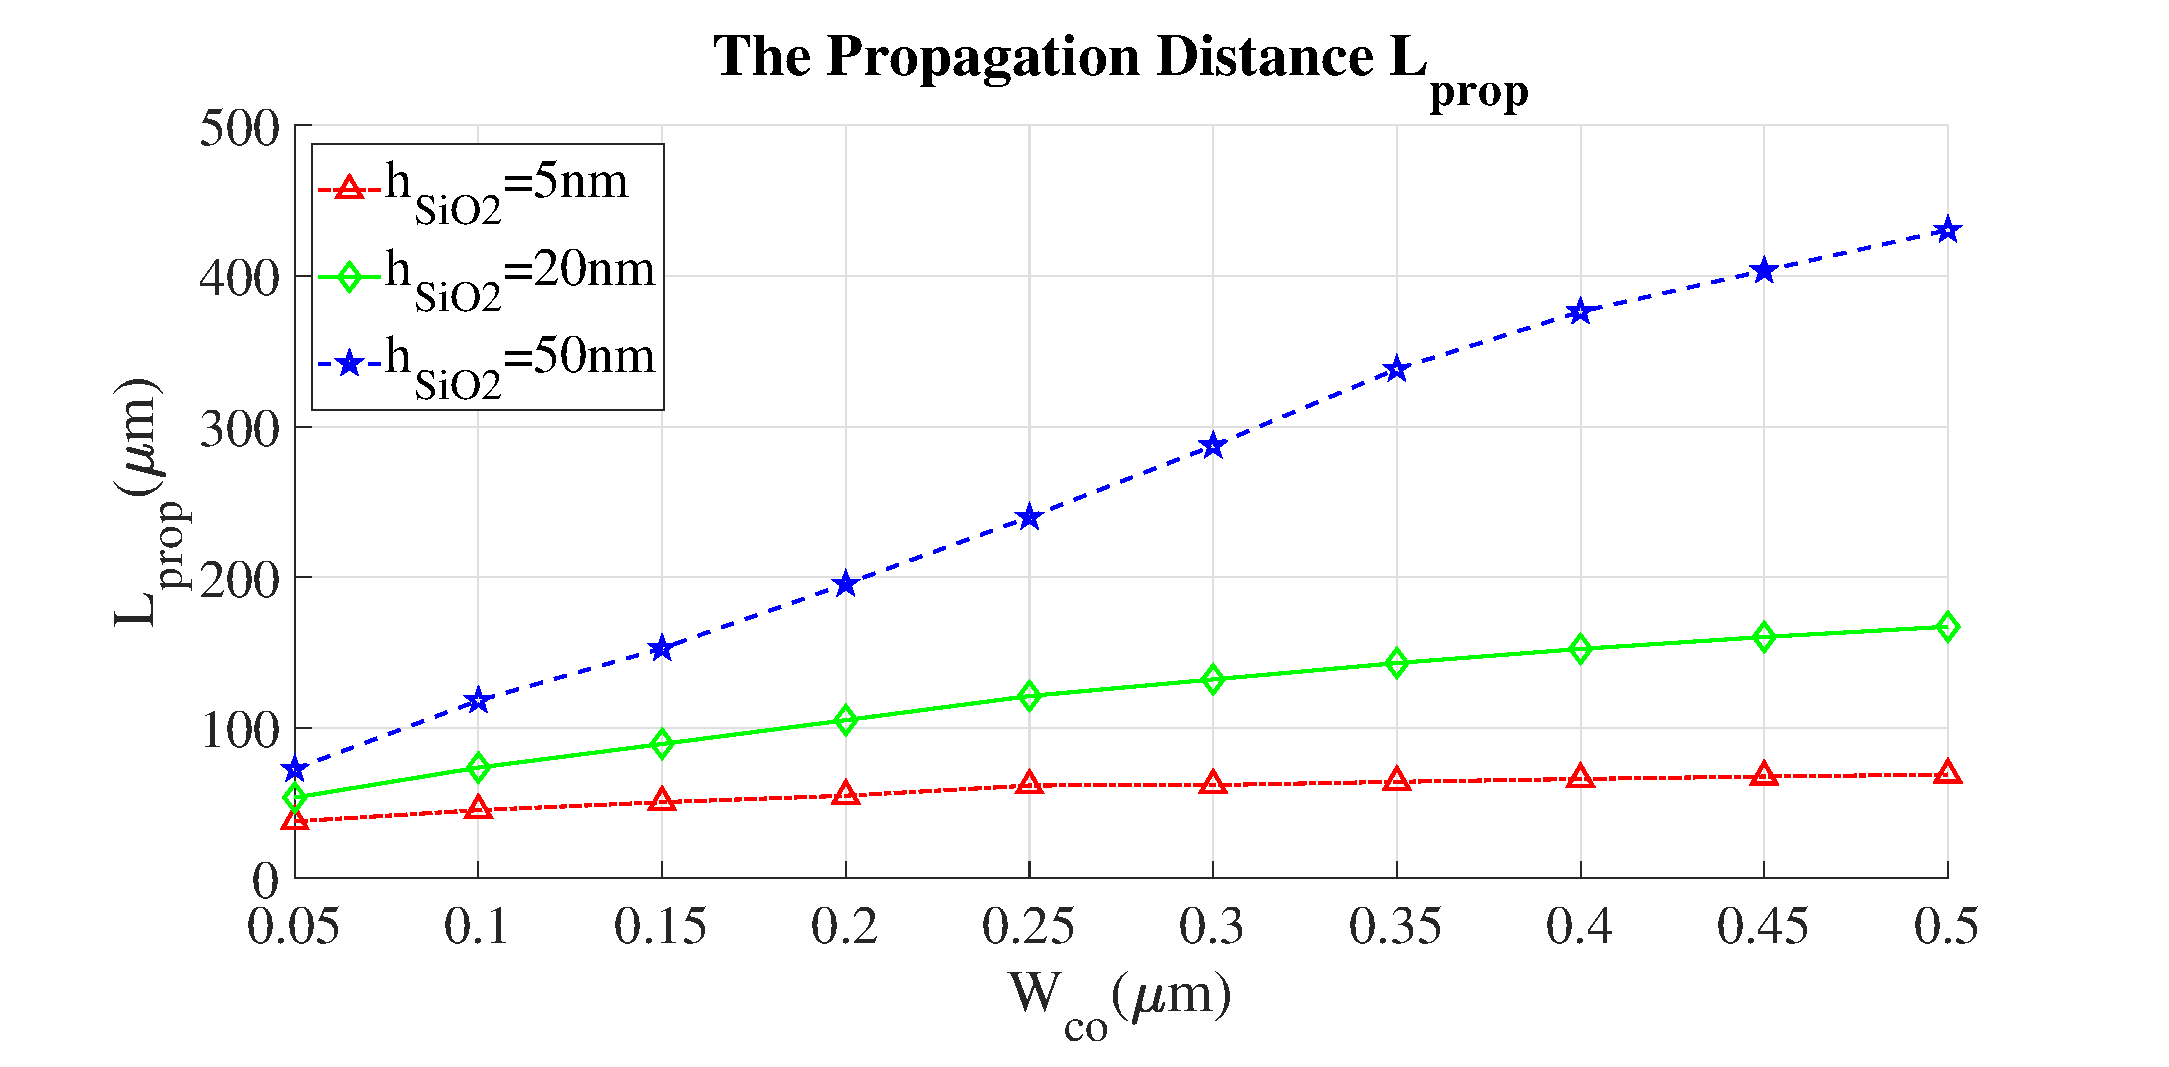
\includegraphics[width=1\textwidth]{nslc_proplen_eps}
	\caption{The propagation length $L_\text{prop}$ for $h_\text{SiO2}$ = 5nm, 20nm, and 50nm.}
	\label{fig:nslc_proplen}
\end{figure}

In summary, the calculation results in Fig.~\ref{fig:nslc_neffr} and ~\ref{fig:nslc_proplen} show that the present hybrid plasmonic waveguide supports a propagation distance on the order of several tens of wavelength $\uplambda$, which is useful to develop plasmonic waveguide devices. One should note that there is a trade-off between the dimension of the plasmon waveguide and its propagation distance.

\subsection{HMIM Plasmonic Waveguide}
The simulation results of the HMIM multilayered plasmonic waveguide described in the Section~\ref{subsubsec:hmim_pw} are shown in here. Mode is confined in both spacer layers.

Fig.~\ref{fig:hmim-neffr} and ~\ref{fig:hmim-neffi} contain the real and imaginary part of the effective mode index of HMIM waveguide for different thickness of spacer and high-dielectric layers respectively. Fig.~\ref{fig:hmim-proplen} shows the propagation length plot of HMIM waveguide for different spacer and high-dielectric layer thickness. Maximum propagation length of 260$\upmu \text{m}$ has been observed at t\_h=300nm, t\_s=200nm.

\begin{figure}[!t]
	\centering
	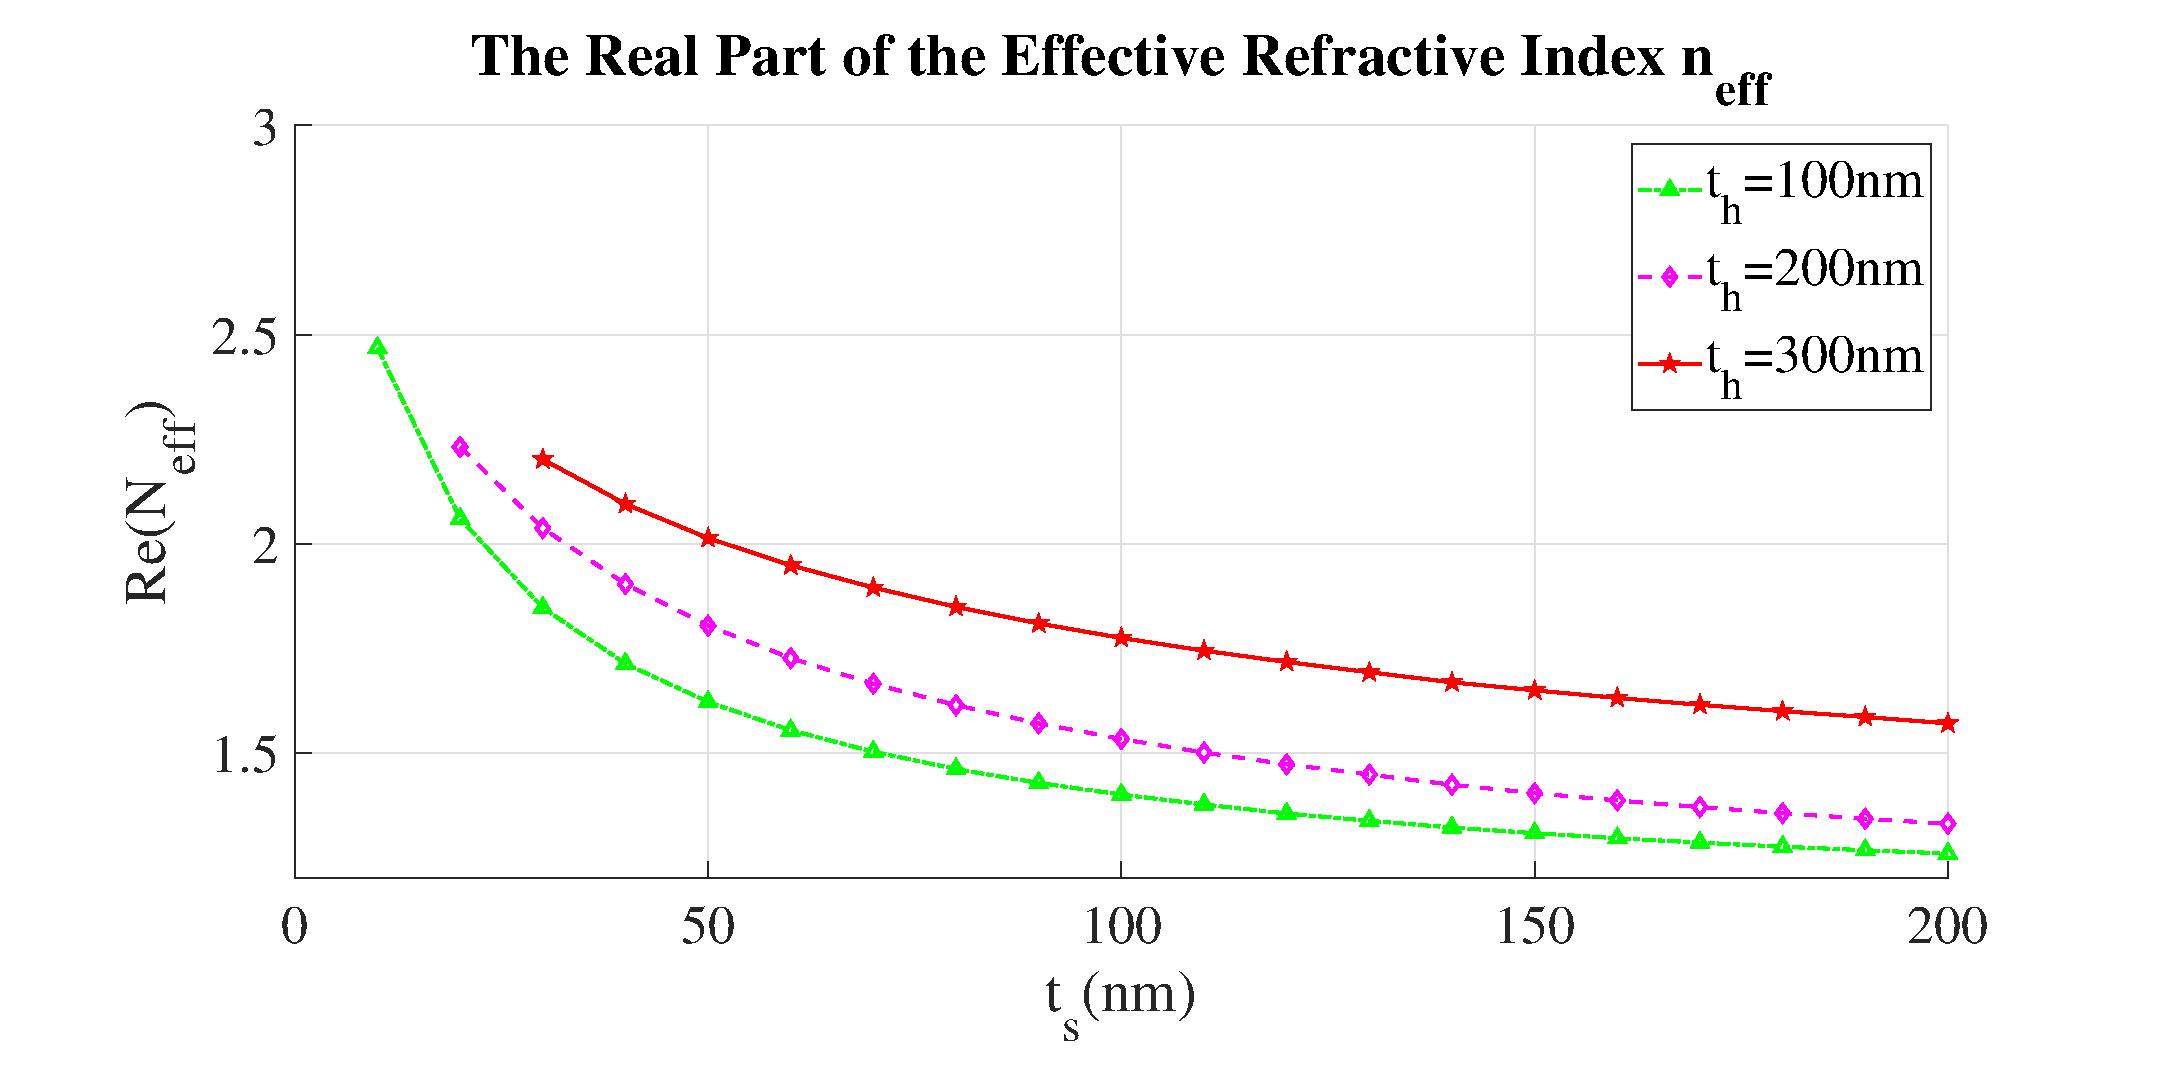
\includegraphics[width=1\textwidth]{hmim-neffr-eps}
	\caption{Real part of effective mode index of hybrid metal insulator metal (HMIM) waveguide.}
	\label{fig:hmim-neffr}
\end{figure}

\begin{figure}[!t]
	\centering
	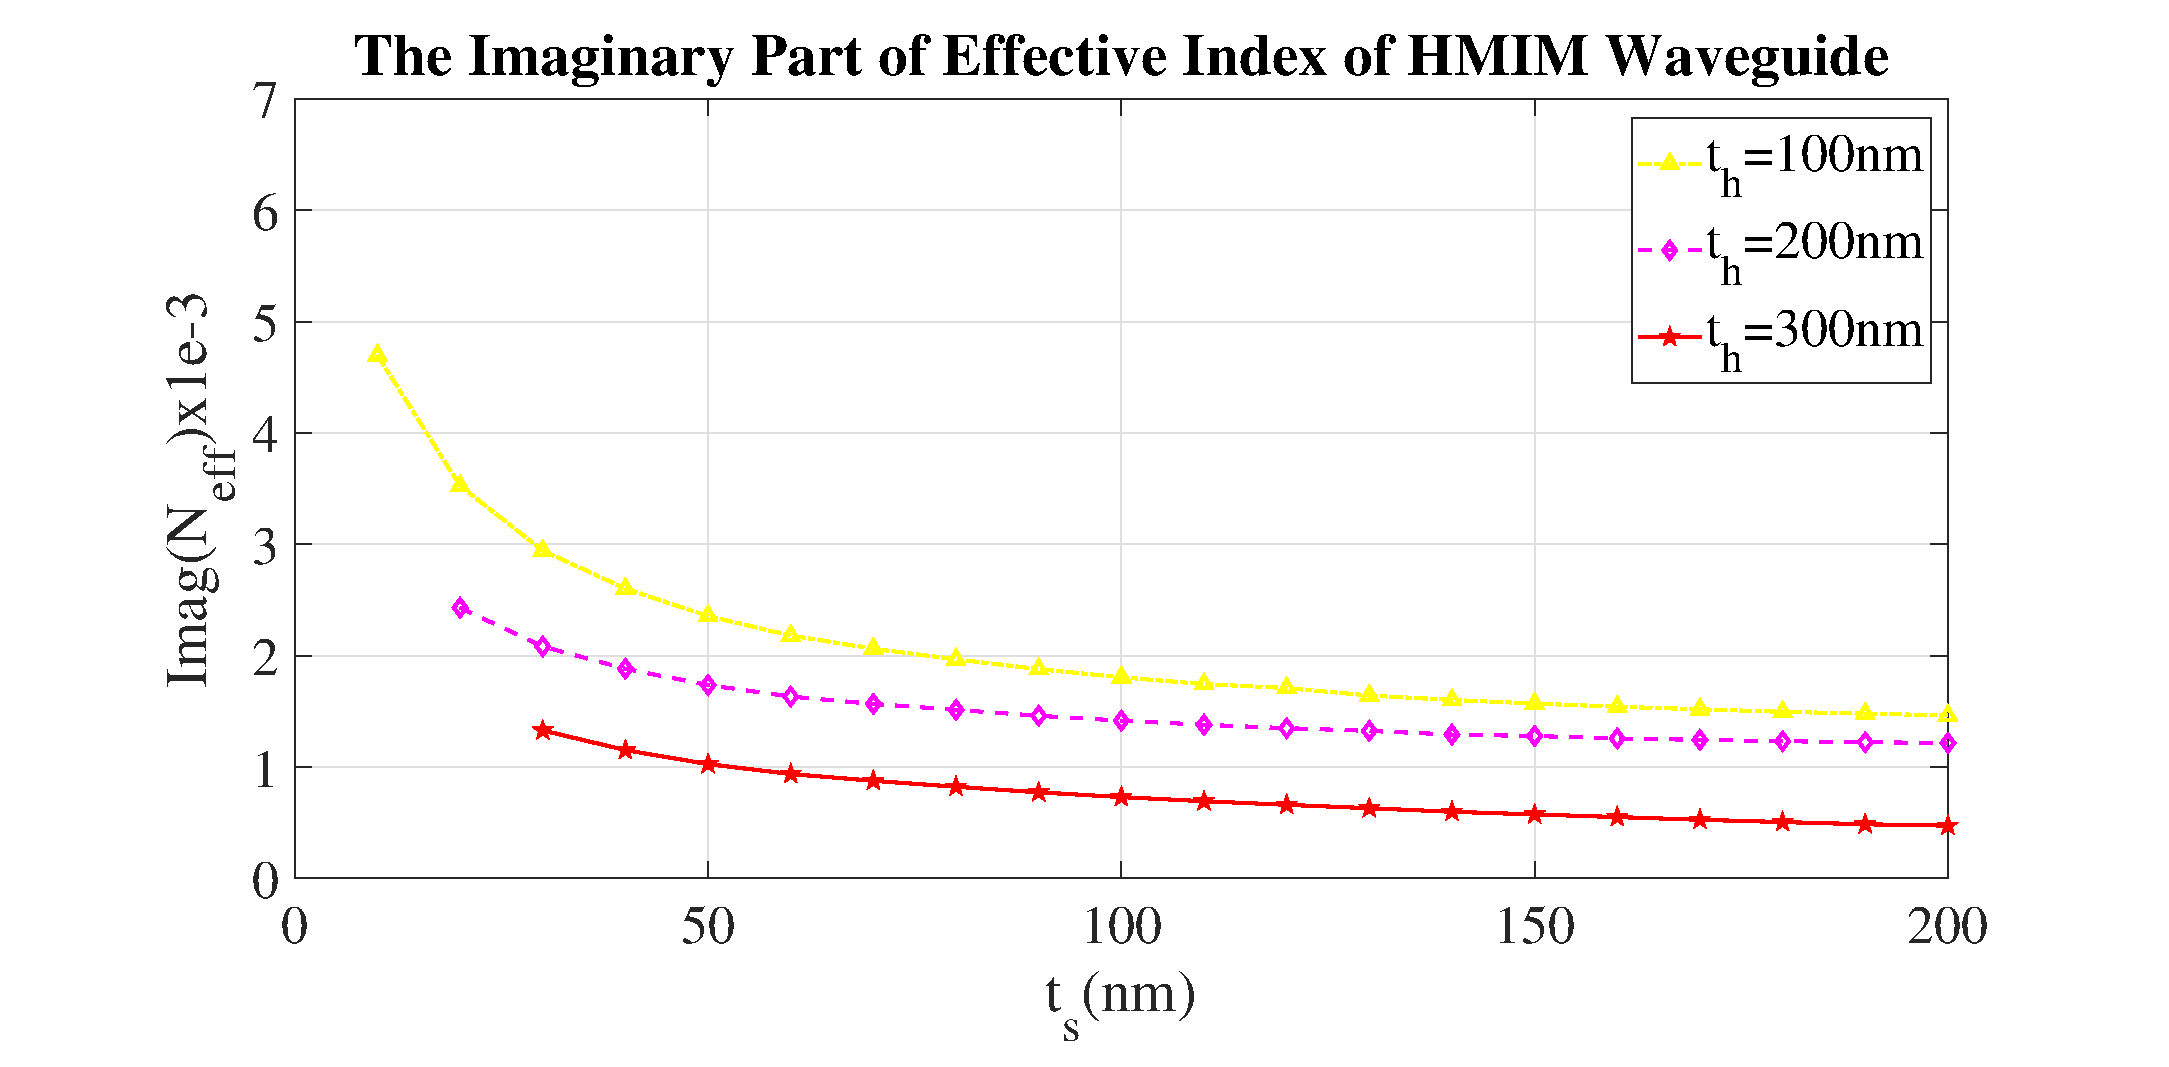
\includegraphics[width=1\textwidth]{hmim-neffi-eps}
	\caption{Imaginary part of effective mode index of hybrid metal insulator metal (HMIM) waveguide.}
	\label{fig:hmim-neffi}
\end{figure}

\begin{figure}[!t]
	\centering
	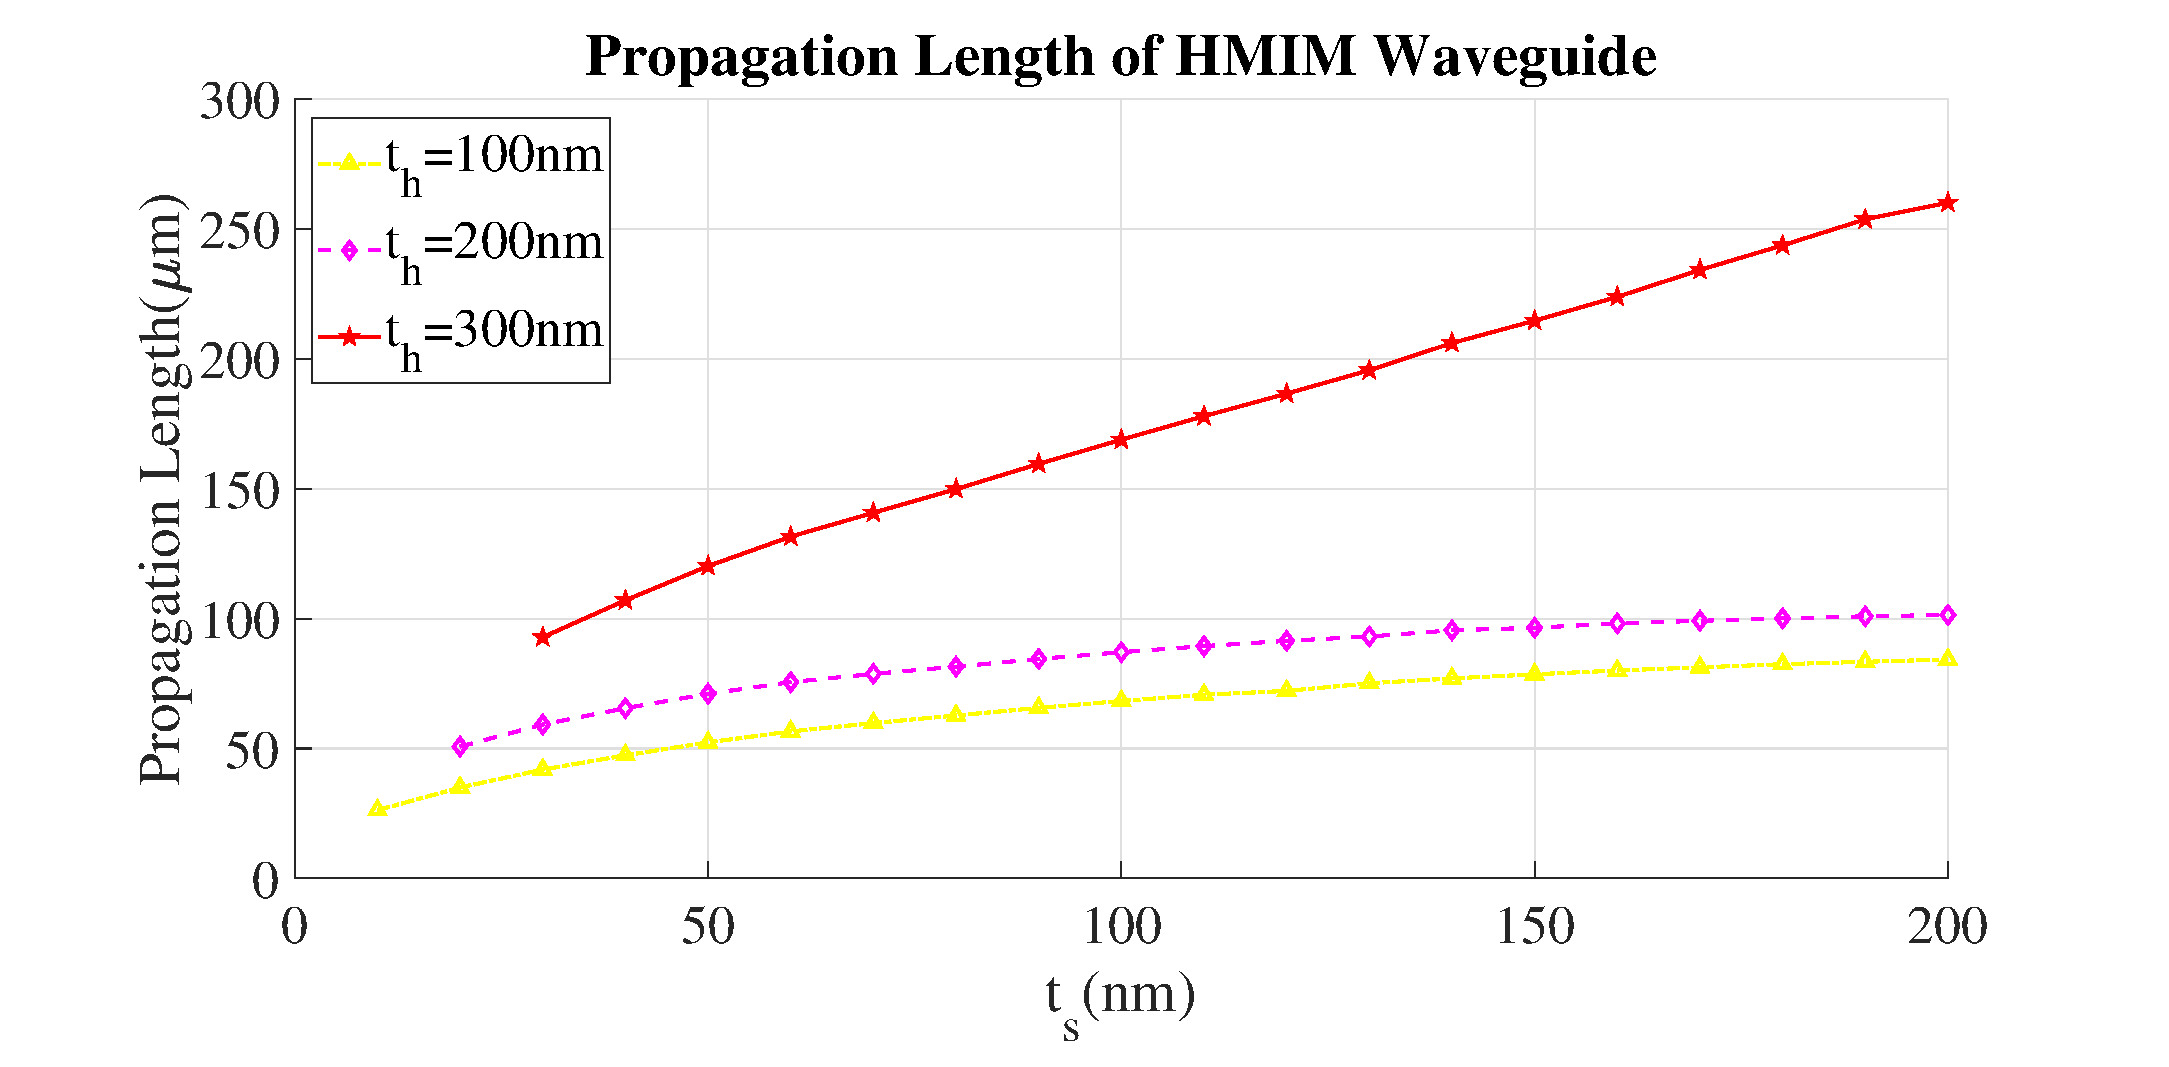
\includegraphics[width=1\textwidth]{hmim-proplen-eps}
	\caption{Propagation length of hybrid metal insulator metal (HMIM) waveguide.}
	\label{fig:hmim-proplen}
\end{figure}

\subsection{InP-based HP-Waveguide}
The InP-based deeply etched hybrid plasmonic waveguide consists of an InGaAsP core layer with a thickness of 500 nm and a bandgap energy of 0.992 eV (equal to a bandgap wavelength of 1.25 $\mu$m) denoted as Q(1.25), an InP cladding layer with a thickness of 160 nm on a semi-insulating InP substrate. The layer stack of hybrid plasmonic waveguide is capped by gold (Au) or silver (Ag) with a thickness of 110 nm. The thickness of the capped metal is optimized during the simulation of passive devices to enhance the power transmission from an input waveguides into the output waveguide. The refractive index of InGaAsP (Q(1.25)), InP, and gold (Au) are equal to 3.3636, 3.1669, and 0.187 + 10.3457i, respectively, at a wavelength of 1550 nm~\cite{Nikoufard2017}.

Mode profile of InP-based HP-waveguide is shown in Fig.~\ref{fig:InP_hpw_modeprofile}. Fig.~\ref{fig:MMI_neffr} shows the real part of effective refractive index of the first five TM modes at the wavelength of 1.55 $\mu$m for the HP-waveguide. In the HP-waveguide, the fundamental $\text{TM}_{00}$ mode does not exhibit a cutoff, and the number of modes supported by the HP-waveguide increases with the width of the ridge. The cutoff widths for $\text{TM}_{01}$, $\text{TM}_{02}$, and $\text{TM}_{03}$ modes are equal to 400, 700, and 1200 nm, respectively. The real part of the effective refractive index approaches toward the refractive index of the InGaAsP layer, as the width of the ridge increases.

\begin{figure}[!t]
	\centering
	\includegraphics[width=0.5\textwidth,height=0.3\textheight]{InP_hpw_mode}
	\caption{Mode profile of InP-based HP-waveguide.}
	\label{fig:InP_hpw_modeprofile}
\end{figure}

\begin{figure}[!t]
	\centering
	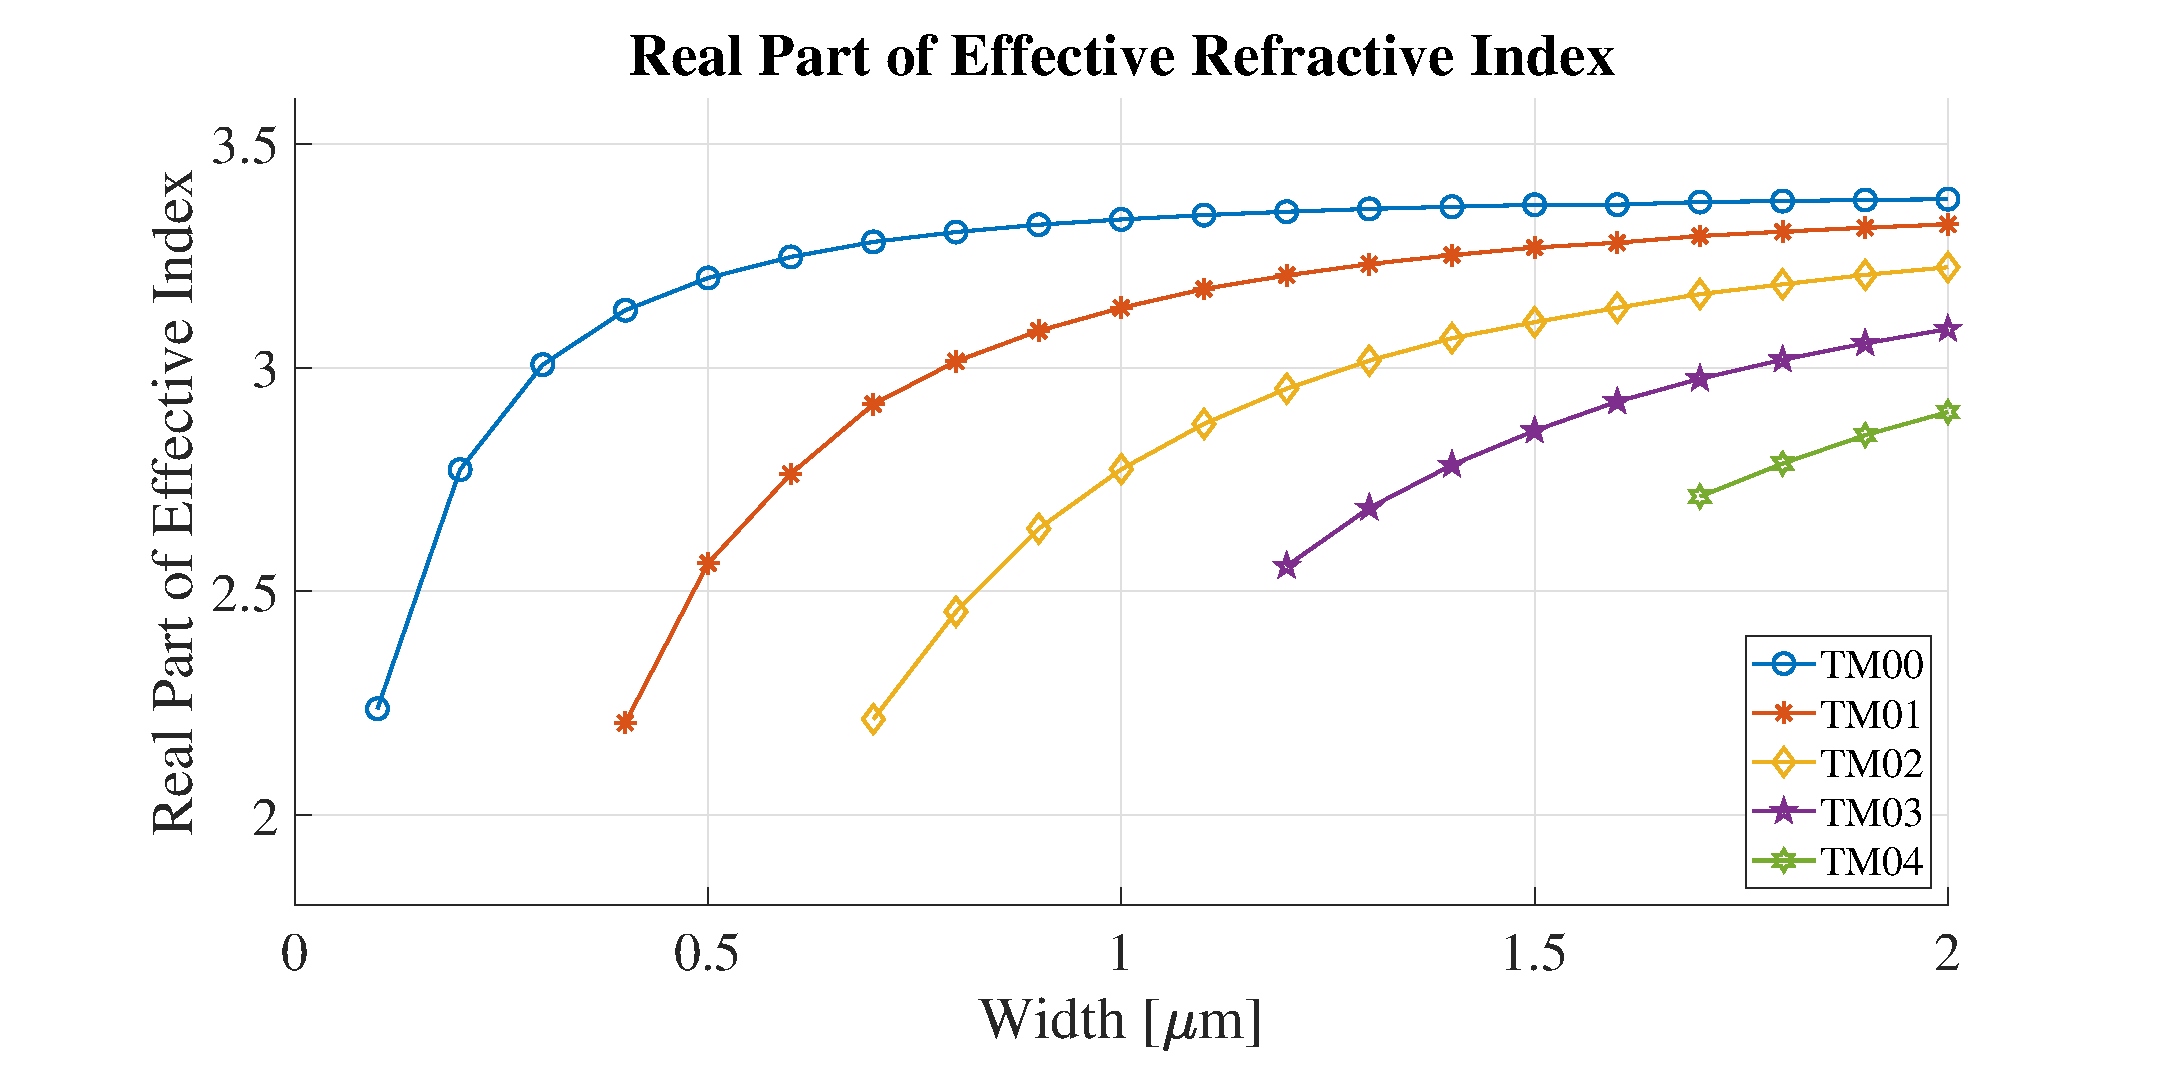
\includegraphics[width=1\textwidth]{MMI_neffr_eps}
	\caption{Real part of effective refractive index for fundamental ($\text{TM}_{00}$), first ($\text{TM}_{01}$), second ($\text{TM}_{02}$), third ($\text{TM}_{03}$), and fourth ($\text{TM}_{04}$) modes, as a function of the width of InP-based HP-waveguide.}
	\label{fig:MMI_neffr}
\end{figure}

\begin{figure}[!t]
	\centering
	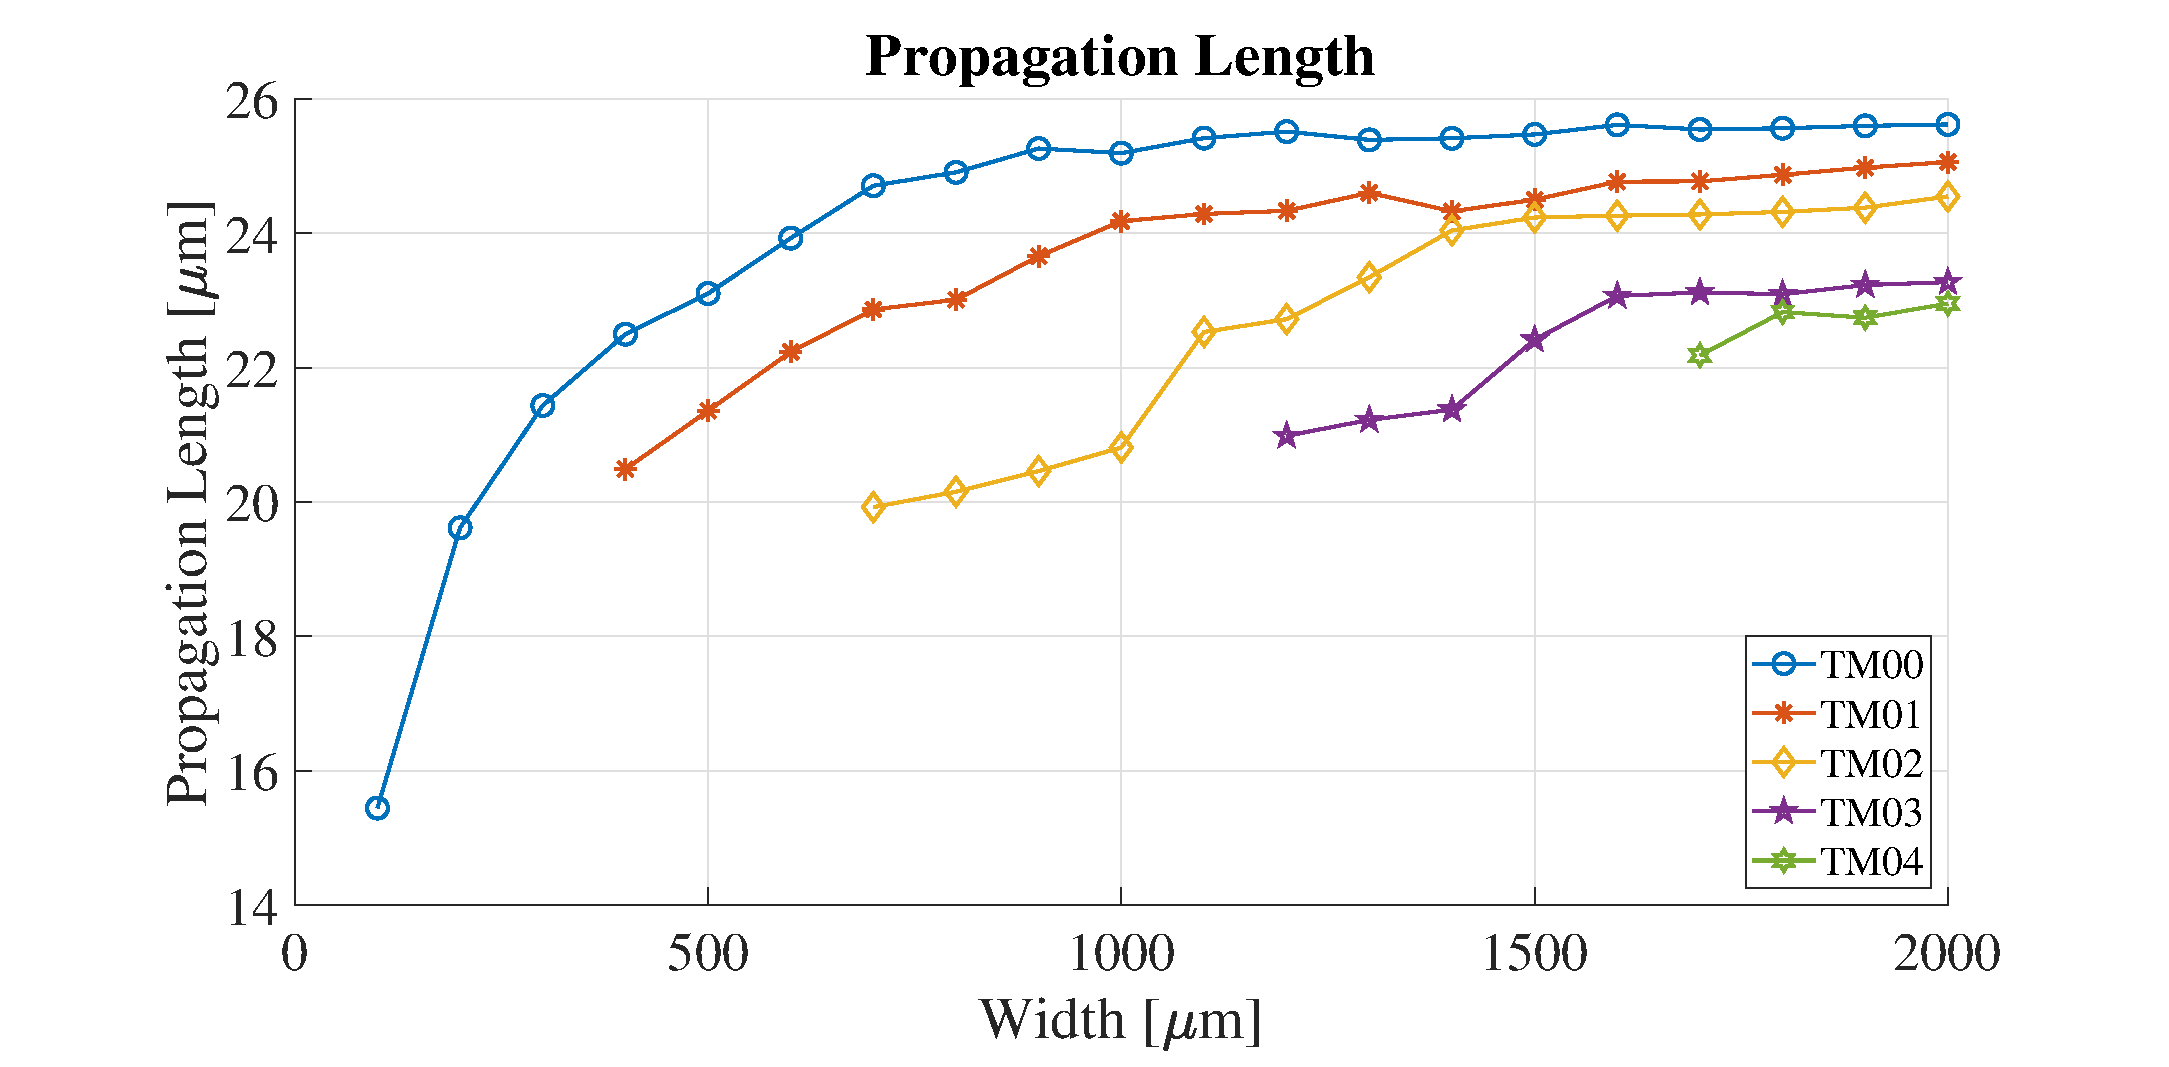
\includegraphics[width=1\textwidth]{MMI_proplen_eps}
	\caption{Propagation length as a function of the InP-based HP-waveguide for $\text{TM}_{00}$, $\text{TM}_{01}$, $\text{TM}_{02}$, $\text{TM}_{03}$, and $\text{TM}_{04}$ modes, determined from the imaginary part of the effective refractive index.}
	\label{fig:MMI_proplen}
\end{figure}

The propagation length of the deeply etched HP-waveguide, determined from the imaginary part of the effective refractive index, i.e., $L_\text{p}$ = $1/(2k_0 n_{\text{eff,imag}})$, where $n_{\text{eff,imag}}$ is the imaginary part of the effective refractive index of the HP waveguide and $k_0 = 2\pi/ \lambda$ is the wavenumber in vacuum. The propagation length for first five TM modes at the wavelength of 1.55 $\mu$m is show in Fig.~\ref{fig:MMI_proplen}.

\section{HPW Devices}
In this section, we present the simulation result of optical ring resonator (ORR) based on  hybrid dielectric-loaded plasmonic waveguide (HDLW). We also discuss the characteristics of SOI-based hybrid plasmonic waveguide horn nanoantenna.

\subsection{Ring Resonator}
Fig.~\ref{fig:hdlw_efield_2000nm_res} and ~\ref{fig:hdlw_efield_2000nm_non_res} show the E-field norm distribution of HDLW-based ring resonator at R = 2000nm for both resonating and non-resonating wavelengths respectively. While, Fig.~\ref{fig:hdlw_efield_5000nm_res} and ~\ref{fig:hdlw_efield_5000nm_non_res} show the E-field norm distribution of HDLW-based ring resonator at R = 5000nm for both resonating and non-resonating wavelengths respectively.  It is clear from the figure that whenever phase is integral multiple of 2$\uppi$, almost entire power is coupled in the ring waveguide and a very negligible amount of power is transmitted at output port. This explains the properties of notch filter i.e., for a range of frequencies, there is a very negligible amount of power transmitted at the output port and most of the power is coupled in the ring waveguide.

The transmission characteristics of ring resonator are shown in the Fig.~\ref{fig:hdlw_transmission}. As it can be seen from the figure that extinction ratio is relatively higher when R = 5 $\upmu\text{m}$ as compared to that of R = 2 $\upmu\text{m}$. This explains the fact that in order to get better (smaller) confinement, we have to trade-off between propagation loss and the confinement area. The values of some important parameters for the simulation of this resonator structure are listed in the table~\ref{tab:rr_params}. These parameters can be changed as per requirement.

\renewcommand{\arraystretch}{1.3}
\begin{table}[!t]
	\begin{center}
		\caption{\label{tab:rr_params} Design Parameters of Ring Resonator.}%\vspace{-2.0mm}
		\scalebox{0.95}{
			\begin{tabular}{ccc}\hline
				Parameter 	&	Value	&	Description\\ \hline 
				R 			& 2 or 5 $\upmu\text{m}$ & Ring radius\\ \hline 
				g 			& 200 or 150 nm & Gap distance\\ \hline
				t$_{\text{SiO}_2}$	& 50 nm & $\text{SiO}_2$ thickness\\ \hline
				t$_{\text{Si}}$	& 150 nm & Si thickness\\ \hline
				t$_{\text{Ag}}$	& 100 nm & Ag thickness\\ \hline
				W			& 300 nm & Waveguide width\\ \hline
				N$_{\text{Si}}$ & 3.4785 & Si refractive index\\ \hline
				N$_{\text{SiO}_2}$	& 1.4491 & $\text{SiO}_2$ refractive index\\ \hline
				N$_{\text{Ag}}$ & 0.1453 +11.3587i & Ag refractive index\\ \hline
			\end{tabular}
		}%\vspace{-3mm}
	\end{center}
\end{table}

\begin{figure}[!t]
	\centering
	\includegraphics[width=1\textwidth]{hdlw_normE_dist_2000nm_res}
	\caption{E-field norm distribution of HDLW based ring resonator at resonating wavelength $(\lambda = 1.58 \mu m)$.}
	\label{fig:hdlw_efield_2000nm_res}
\end{figure}

\begin{figure}[!t]
	\centering
	\includegraphics[width=1\textwidth]{hdlw_normE_dist_2000nm_non_res}
	\caption{E-field norm distribution of HDLW based ring resonator at non-resonating wavelength $(\lambda = 1.60 \mu m)$.}
	\label{fig:hdlw_efield_2000nm_non_res}
\end{figure}

\begin{figure}[!t]
	\centering
	\includegraphics[width=1\textwidth]{hdlw_normE_dist_5000nm_res}
	\caption{E-field norm distribution of HDLW based ring resonator at resonating wavelength $(\lambda = 1.592 \mu m)$.}
	\label{fig:hdlw_efield_5000nm_res}
\end{figure}

\begin{figure}[!t]
	\centering
	\includegraphics[width=1\textwidth]{hdlw_normE_dist_5000nm_non_res}
	\caption{E-field norm distribution of HDLW based ring resonator at non-resonating wavelength $(\lambda = 1.58 \mu m)$.}
	\label{fig:hdlw_efield_5000nm_non_res}
\end{figure}

\begin{figure}[!t]
	\centering
	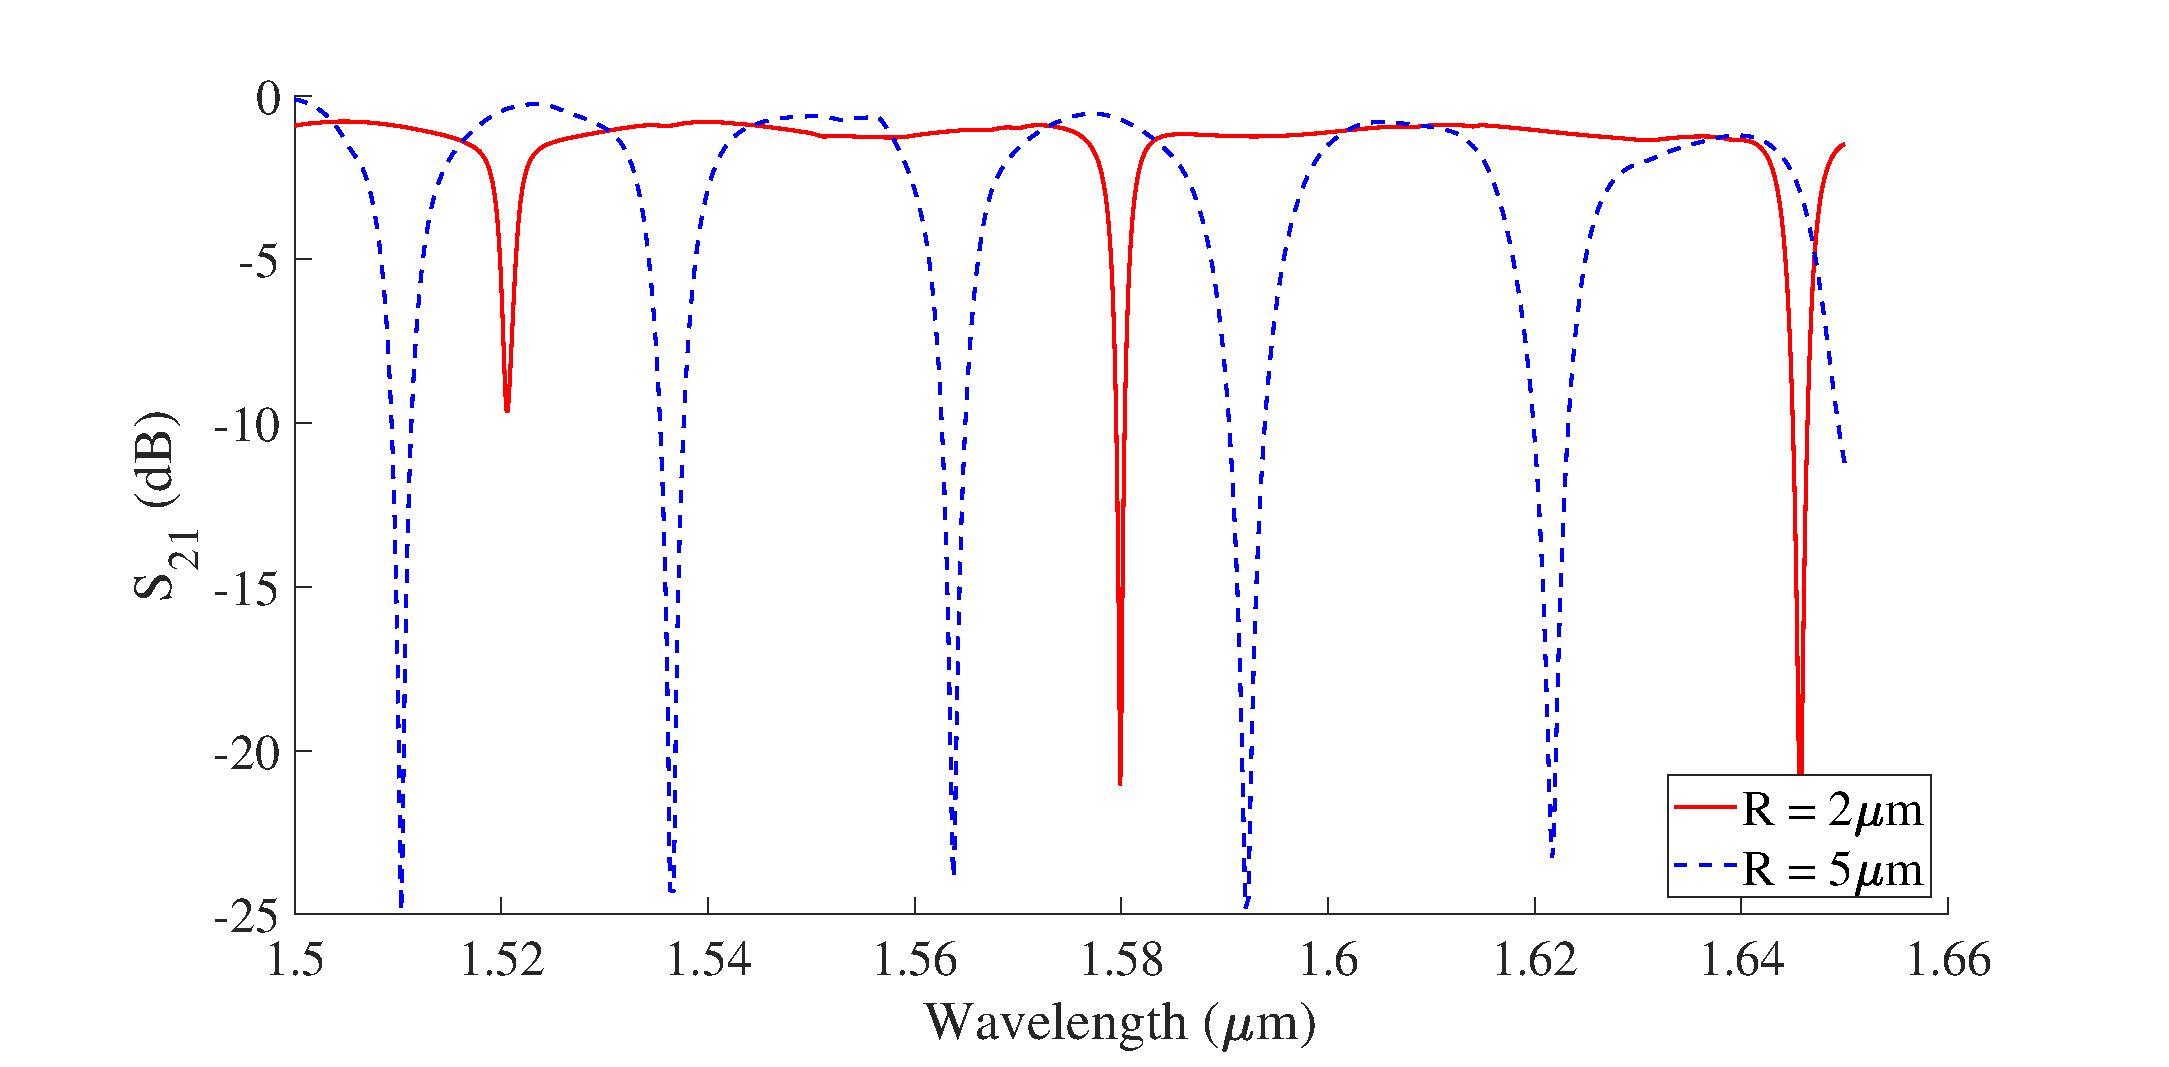
\includegraphics[width=1\textwidth]{hdlw_scatt_param_plot.eps}\vspace{1mm}
	\caption{{Transmission characteristics of HDLW based ring resonator.}}%\vspace{-3mm}
	\label{fig:hdlw_transmission}
\end{figure}

\subsection{Horn-nanoantenna}
Fig.~\ref{fig:hnano_mode_prof} shows that the $\text{SiO}_2$-cladding layer is sandwiched between a metal cap layer and a partly-etched Si layer. The thicknesses of these layers were set at $h_\text{WG}$= 30 nm, $h_\text{Au}$ = 70 nm, and $h_\text{RIB}$ = 100 nm, respectively. The layered structure is taken from~\cite{Yousefi2012} in which the authors have proposed a rectangular patch optical nanoantenna to radiate the optical field from a hybrid plasmonic waveguide.

Fig.~\ref{fig:hnano_mode_prof} and ~\ref{fig:hnano_efield_dist} show the mode profile and the E-field norm distribution of horn-nanoantenna input HP waveguide. It is observed that mode is confined mostly in $\text{SiO}_2$ layer only.

\begin{figure}[!t]
	\centering
	\includegraphics[width=1\textwidth]{hnano_mode_profile.jpg}\vspace{1mm}
	\caption{{Mode profile of horn-nanoantenna input HP waveguide.}}%\vspace{-3mm}
	\label{fig:hnano_mode_prof}
\end{figure}

\begin{figure}[!t]
	\centering
	\includegraphics[width=1\textwidth]{hnano_normE_dist.jpg}\vspace{1mm}
	\caption{{E-field norm distribution of horn-nanoantenna input HP waveguide.}}%\vspace{-3mm}
	\label{fig:hnano_efield_dist}
\end{figure}

	\chapter{Conclusion and Future Work}
	%\linespread{1.5} \normalsize
\section{Conclusion}
This report has discussed the characteristics of hybrid plasmonic (HP) waveguides (HPWs) and their potential applications such as optical ring resonators and nanoantenna. The objectives of this project were to study the properties of various structures of HP-waveguides and to use those structures for different devices used in photonic integrated circuits. Both objectives were met. Three different structures of HP-waveguides were simulated and their characteristics were studied at optical communication wavelength of $\uplambda = \text{1550 nm}$. Adding further to that, an optical ring resonator notch filter based on hybrid dielectric-loaded plasmonic waveguide (HDLW) was simulated and its transmission characteristics were studied at both constructive and destructive interference wavelengths. A high extinction ratio of 22.5 dB and 24.9 dB is obtained at r = 2 $\upmu \text{m}$ and 5 $\upmu \text{m}$ respectively. While low transmission loss of 0.8 dB and 0.5 dB is obtained at radii 2 $\upmu \text{m}$ \& 5 $\upmu \text{m}$ respectively. We also investigated a horn-shaped nanoantenna based on HP-waveguide with silicon-on-insulator (SOI) configuration and its input HP-waveguide was simulated. All simulations were carried out using finite element method (FEM) in COMSOL Multiphysics software and graphs were plotted with the help of MATLAB.

\section{Future Work}
In future, we would like to investigate hybrid plasmonic waveguides of other potential applications such as biosensors and optical switches. Also, we would like to extend our work on optical ring resonators to simulate different kind of optical filters with better extinction ratio and low loss.
	
	
	\newpage
	% The bibliography goes under a separate .bib file. To quote articles, just fill the appropriate headings in the bibliography file.
	\addcontentsline{toc}{chapter}{References}
%	\bibliographystyle{unsrt}
%	\bibliographystyle{IEEEtran}
	\bibliographystyle{apalike}
	\bibliography{reference_ev}
	
	\begin{appendices}
		\addtocontents{toc}{\protect\setcounter{tocdepth}{0}}
		\chapter{Formulae and Derivations}
		\section{Evanescence in waveguides}
In all optical fibers, light propagates by means of total internal reflection, wherein the propagating light is launched into waveguide at angles such that upon reaching the cladding-core interface, the energy is reflected and remains in the core of the fiber. Remarkably, however, for light reflecting at angles near the critical angle, a significant portion of the power extends into the cladding or medium which surrounds the core. This phenomenon, known as the evanescent wave, extends only to a short distance from the interface, with power dropping exponentially with distance. A detailed discussion can be found in~\cite{Anderson2008}.

\section{Finite Element Method}
The finite element method (FEM) is a numerical technique for solving problems which are described by partial differential equations or can be formulated as functional minimization. A domain of interest is represented as an assembly of finite elements. Approximating functions in finite elements are determined in terms of nodal values of a physical field which is sought. A continuous physical problem is transformed into a discretized finite element problem with unknown nodal values. For a linear problem a system of linear algebraic equations should be solved. Values inside finite elements can be recovered using nodal values. For a detailed discussion on FEM, visit \href{https://www.comsol.co.in/multiphysics/finite-element-method}{COMSOL} official website.




	\end{appendices}
	
	
	
\end{document}